\chapter{Teledetección}

\section{Introducción a la teledetección}

\subsection{Historia de la Fotogrametría y Teledetección}

\subsubsection{Fotogrametría}

El desarrollo de las matemáticas como disciplina de la lógica
no existía hasta antes del año 1000 a.C.
El filósofo griego Aristóteles (-350 a.C.) se refirió al
proceso de proyección óptica de imágenes. Leonardo
da Vinci exploró las disciplinas de la óptica,
geometría y mecánica. En 1492 demostró
los \texttt{principios de la perspectiva óptica} (MacLeish
1977), que sienta las bases de
\textbf{fotogrametría} incluso hoy. 

Alberto Durero (1471-1528) en 1525 construyó muestras de dispositivos mecánicos
para hacer dibujos en perspectiva reales de la naturaleza
y escenas de estudio, así como para producir
dibujos \texttt{estereoscópicos} (ASPRS 1980).

El astrónomo Alemán Johannes Kepler en 1600 dio una precisa
definición de estereoscopía. Aughtread de Inglaterra en
1574 desarrolló la primera regla de cálculo y pronto
a partir de entonces, John Napier (1550-1617) publicó tablas
de logaritmos; Blaise Pascal (1623-1662)
estableció el concepto de \texttt{metrología} y dio la
mundo una calculadora de escritorio. 

Isaac Newton (1642-1727) y Gottfried von Leibnitz (1646-1716) firmemente
estableció los conceptos de diferencial y
cálculo integral. Conceptos de central inversa
Resección de perspectiva y espacio de imágenes conjugadas 
fueron discutidos por primera vez por J. Henry Lambert (1728-
1777) en su libro ``Perspectiva Freie'' en 1759.

Wheatstone de Inglaterra, presentó en 1838 el \texttt{estereoscopio}, una de las herramientas más importantes fotogrametría. La práctica de la fotogrametría sólo podría iniciarse después de que Arago y Niepce anunciaron un ``proceso heliográfico'', basado en el cual Louis J.M. Daguerre (1789-1851) presentó a la Academia Francesa de Artes y Ciencias en 1837, fotografías a las que llamó ``daguerrotipos''. los acuñados al término ''fotogrametría'' en 1855 por Kersten con su introducción por Meydenbauer en 1867 a la literatura internacional, el primer  libro de texto alemán sobre fotogrametría de Koppe (1889) y  La obra clásica de Aimé Laussedat sobre fotogrametría francesa (1898) son algunos de los hitos del análisis fotogrametría registrada en la historia (ISPRS 1980).

Hauck (1883) estableció la relación entre la geometría proyectiva y fotogrametría. Esta debe considerarse como el concepto geométrico y la base de la mayoría de los clásicos desarrollos fotogramétricos analíticos.

Ernst Abbe, cofundador de la Zeiss Works alemana en 1871 inició intensos estudios y pruebas para elementos ópticos con base en rigurosos análisis matemáticos. F. Stolze descubrió el principio de la marca flotante en 1892, mientras que Carl Pulfrich, también del grupo Zeiss, desarrolló un método práctico para medir y derivar \texttt{dimensiones de imágenes estereofotografías} con marcas flotantes. Presentó en 1901 el estereocomparador Zeiss Pulfrich complementando a Eduard, el primer prototipo de von Orel (1877-1941) estereoautógrafo en el 73 Congreso de Ciencias Naturales y Medicina celebrado en Hamburgo.

Por separado, se inventó un estereocomparador similar en 1901 por Henry G. Fourcade (1865-1948) en Sudáfrica.  Presentó esto en la Sociedad Filosófica de la Ciudad del Cabo.

Sebastian Finsterwalder (1862-1951) en una serie de
publicaciones durante 1899 a 1937 establecieron una muy
base sólida para la fotogrametría analítica.
En estos provocó las relaciones geométricas
que gobiernan la resección e intersección, así como
orientaciones relativas y absolutas. El predijo
la posibilidad futura de la triangulación del punto nadir
y fotogrametría aplicativa a mediciones astrogeodésicas. Él también formuló las
leyes básicas del \texttt{error de propagación} en triangulaciones de tira larga.
Él fue, posiblemente, la primera persona en utilizar la \texttt{terminología vectorial} en la literatura fotogramétrica (Finsterwalder 1899, 1932).

Eduard Dalezal (1862-1955) de Viena, Austria
brindó un gran espíritu impulsor internacional mientras
que se convirtió en el presidente de la Sociedad Internacional
de Fotogrametría en 1909. Él también.
creó los Archivos Internacionales de la
Fotogrametría.

Los revolucionarios desarrollos tecnológicos que
comenzó en la década de 1970 en campos como
microelectrónica, semiconductores y
la fotónica ha influido en nuevos pensamientos fundamentales
e investigaciones encaminadas a obtener mejores
eficiencias en el registro, procesamiento de datos,
fases de almacenamiento y administración de datos de
operaciones fotogramétricas. En informática,
un sistema ``en tiempo real'' se entiende como ``el
procesamiento de información o datos de una 
manera lo suficientemente rápida como para que 
los resultados del procesamiento estén disponibles
a tiempo para influir en el proceso que se está 
monitoreando o controlando (Sipple 1972).

El desarrollo histórico de los instrumentos en
La fotogrametría analítica se puede ver con respecto
a las siguientes agrupaciones (componente funcional
relacionado):

\begin{enumerate}
    \item Instrumentos para la adquisición de datos (que comprenden
    comparadores, marcado y transferencia de puntos
    dispositivos).
    \item Instrumentos para el procesamiento de datos (que comprenden
    trazadores de imágenes espaciales, trazadores analíticos y
    trazadores híbridos o convertidos).
    \item Instrumentos para visualización y presentación de datos
    (que comprende tablas de trazado, sistemas de software
    y ortofotoimpresoras).
\end{enumerate}


\subsubsection{Teledetección}

En 1859, Gaspard Tournachon tomó una fotografía oblicua de un pequeño pueblo cerca de París desde un
globo. Con esta imagen había comenzado la era de la observación de la tierra y la teledetección. Su
Pronto el ejemplo fue seguido por otras personas de todo el mundo. Durante la Guerra Civil en el
La fotografía aérea de Estados Unidos desde globos jugó un papel importante para revelar la defensa.
puestos en Virginia. Asimismo, otros desarrollos científicos y técnicos de esta Guerra Civil
El tiempo en los Estados Unidos aceleró el desarrollo de la fotografía, lentes y aplicaciones
uso aerotransportado de esta tecnología. Aunque la era espacial de la teledetección aún estaba muy lejos
Después de la Guerra Civil, ya en 1891 se concedieron patentes en Alemania a diseños exitosos de
cohetes con sistemas de imágenes bajo el título: ``Aparato nuevo o mejorado para obtener aves
vistas fotográficas del ojo de la Tierra ”. El diseño comprendía un sistema de cámara propulsada por cohete.
que fue recuperado por un paracaídas. La Tabla 1.1 muestra algunas fechas importantes en el desarrollo
de la teledetección.

El siguiente período de rápido desarrollo tuvo lugar en Europa y no en los Estados Unidos. Era durante la Primera Guerra Mundial, los aviones se utilizaron a gran escala para el reconocimiento fotográfico.
Las aeronaves demostraron ser plataformas más confiables y estables para la observación de la Tierra que
globos. En el período comprendido entre la Primera Guerra Mundial y la Segunda Guerra Mundial se inició con el
uso de fotografías aéreas. Los campos de aplicación de las fotos aerotransportadas incluían en ese momento la geología,
silvicultura, agricultura y cartografía. Estos desarrollos conducen a cámaras muy mejoradas,
películas y equipo de interpretación. Los desarrollos más importantes de la fotografía aérea

y la interpretación de fotografías tuvo lugar durante la Segunda Guerra Mundial. Durante este lapso de tiempo el
desarrollo de otros sistemas de imágenes, como fotografía de infrarrojo cercano, detección térmica
y tuvo lugar el radar. La fotografía de infrarrojo cercano y el infrarrojo térmico resultaron muy valiosos para
separar la vegetación real del camuflaje. El primer radar de imágenes aerotransportado exitoso no fue
utilizado con fines civiles, pero resultó valioso para bombardeos nocturnos. Como tal, el sistema
fue llamado por el ``indicador de posición del plan'' militar y fue desarrollado en Gran Bretaña en
1941.

Después de las guerras de la década de 1950, los sistemas de teledetección continuaron evolucionando a partir de los sistemas
desarrollado para el esfuerzo de guerra. Se descubrió que la fotografía infrarroja en color (CIR) es de gran utilidad
para las ciencias vegetales. En 1956 Colwell llevó a cabo experimentos sobre el uso de CIR para
la clasificación y reconocimiento de tipos de vegetación y la detección de enfermedades y
vegetación dañada o estresada. También fue en la década de 1950 cuando los avances significativos en el radar
se logró la tecnología. En ese momento se desarrollaron dos tipos de radar: SLAR: radar aerotransportado con vista lateral, y SAR: radar de apertura sintética. Cualquiera de los desarrollos dirigidos a la
adquisición de imágenes con la mayor resolución posible. Crucial para el desarrollo del SAR fue
la capacidad de resolver con precisión las frecuencias Doppler utilizando un algoritmo de análisis de frecuencia en
la señal de radar que regresa del centro de investigación de la Fuerza Aérea de EE. UU.

\subsection{Radiación Electromagnética}

La Teledetección estudia las características físicas de un cuerpo usando la radiación que emite el cuerpo captado con un sensor, sin necesidad de estar en contacto físico. 

\begin{definition}[Satelites]
    Son vehículos artificiales puestos en órbitas alrededor de la tierra o otros planetas y asteroides, llevan a bordos equipos e instrumentos científicos para realizar tareas definidas. 
    Según el propósitos por el cual fueron diseñados, los satélites se clasifican en: 
    \begin{itemize}
        \item \textbf{Satélites de comunicaciones}: (órbitas geosíncronas a 36,000km)
        \item \textbf{Satélites de la Tierra}: Para la observación de la tierra, llevan a bordo sensores terrestres. Son varios y producen imágenes digitales tales como Landsat, SPOT, WorlfWiev, etc. Sus órbitas están entre 700 a 1400 km 
        \item \textbf{Satélites de geoposicionamiento}: Con órbitas entre 10,000 de 20,500 km, son los que se utilizan para la georreferenciación de los satélites.
        \item \textbf{Satélites meteorológicos}: Con órbitas geosíncronas 
    \end{itemize}
\end{definition}

El espectro electromagnético en término de longitud de onda ($\mu m$) y de frecuencia $GH_z$
\begin{align*}
    1\mu m=10^{-4}cm\\ 
    1nm=10^{-7}cm=10^{-3}\mu m\\ 
    1Hz=1cps\\ 
    1KHz=10^3Hz\\ 
    1GHz=10^{3}KHz
\end{align*}

Las principales regiones del espectro electromagnético dentro del rango comprendido entre $0.20$ y $4.0\mu m$ son: 
\begin{itemize}
    \item Ultravioleta: $0.20\mu m$ a $0.39\mu m$
    \item Visible: $0.39\mu m$ a $0.78\mu m$
    \item Cercano Infrarrojo: $0.78\mu m$ a $4.0\mu m$
    \item Infrarrojo: $4.0\mu m$ a $100000\mu m$
\end{itemize}

Los componentes de una onda electromagnética tiene dos componentes que son mutuamente ortogonales, uno es el campo eléctrico y el otro es el campo magnético
ambos campos tienen la misma amplitud y alcanza su máxima/mínima al mismo tiempo

\subsubsection{Leyes de la Radiación}

\textbf{Ley de Kirchhoff}

La relación entre la radiación emitida y el flujo de la radiación absorbida es lo mismo para todos los cuerpos negros a la misma temperatura. De ahí la definición de la emisividad ($\epsilon$)
como la relación entre emitancia de objeto $M$ y la emitancia de un cuerpo negro $Mn$ a la misma temperatura.

\begin{itemize}
    \item $\epsilon=\frac{M}{Mn}$
    \item $\epsilon=1$ para un cuerpo negro verdadero
    \item $\epsilon=0$ para un reflector perfecto
\end{itemize}

\textbf{Ley de Stefan- Boltzmann} La radiación emitida por un cuerpo negro es proporcional a su temperatura absoluta elevada
a la potencia cuatro.
\begin{equation}
    W=\sigma T^4
\end{equation}

Donde $\sigma=5.6697\times 10^{-8} watt\cdot m^{-2}K^{-4}$ (Constante de Stefan- Boltzmann)

\textbf{Ley de desplazamiento de Wien} Especifica la relación entre la longitud de onda de la radiación emitida y la $T$ absoluta del cuerpo

\begin{equation}
    \lambda=\frac{2897}{T}
\end{equation}


Fuera de la atmósfera terrestre, la radiación solar tiene una intensidad de aproximadamente 1370 $watts/m^2$. Este valor medido en la distancia media sol/tierra, al tope de la atmósfera, es referida como constante solar. En la superficie de la tierra al medio día y la radiación de rayos directos será aproximadamente $1000 watts/m^2$ en varios lugares.

La disponibilidad de la energía solar, están afectada por varios factores como localización (latitud, longitud y altitud), la estación y el tiempo del día. Pero el factor más importante, el más grande es la cobertura de nubes y otras condiciones meteorológicas.
que varían con la localización y el tiempo

Aproximadamente el 99\% de la radiación solar en la superficie de la tierra se concentra en la región de RM entre 0.3 y $3.0\mu m$, mientras que la mayoría de la radiación emitida de superficie terrestre localiza en la región comprendida entre 3.5 a $50\mu m$.
Los efectos atmosféricos sobre la radiación EM son:
\begin{itemize}
    \item Difracción 
    \item Absorción
    \item Refracción
    \item Ventana atmosférica
\end{itemize}

Aproximadamente el 99\% de la radiación solar en la superficie de la tierra se concentra en la región de EM entre 0.3 y 3.0 $\mu m$,
mientras que la mayoría de la radiación emitida de superficie terrestre se localiza en la región comprendida entre 3.5 a 50 $\mu m$.

\begin{figure}[h!]
  \centerline{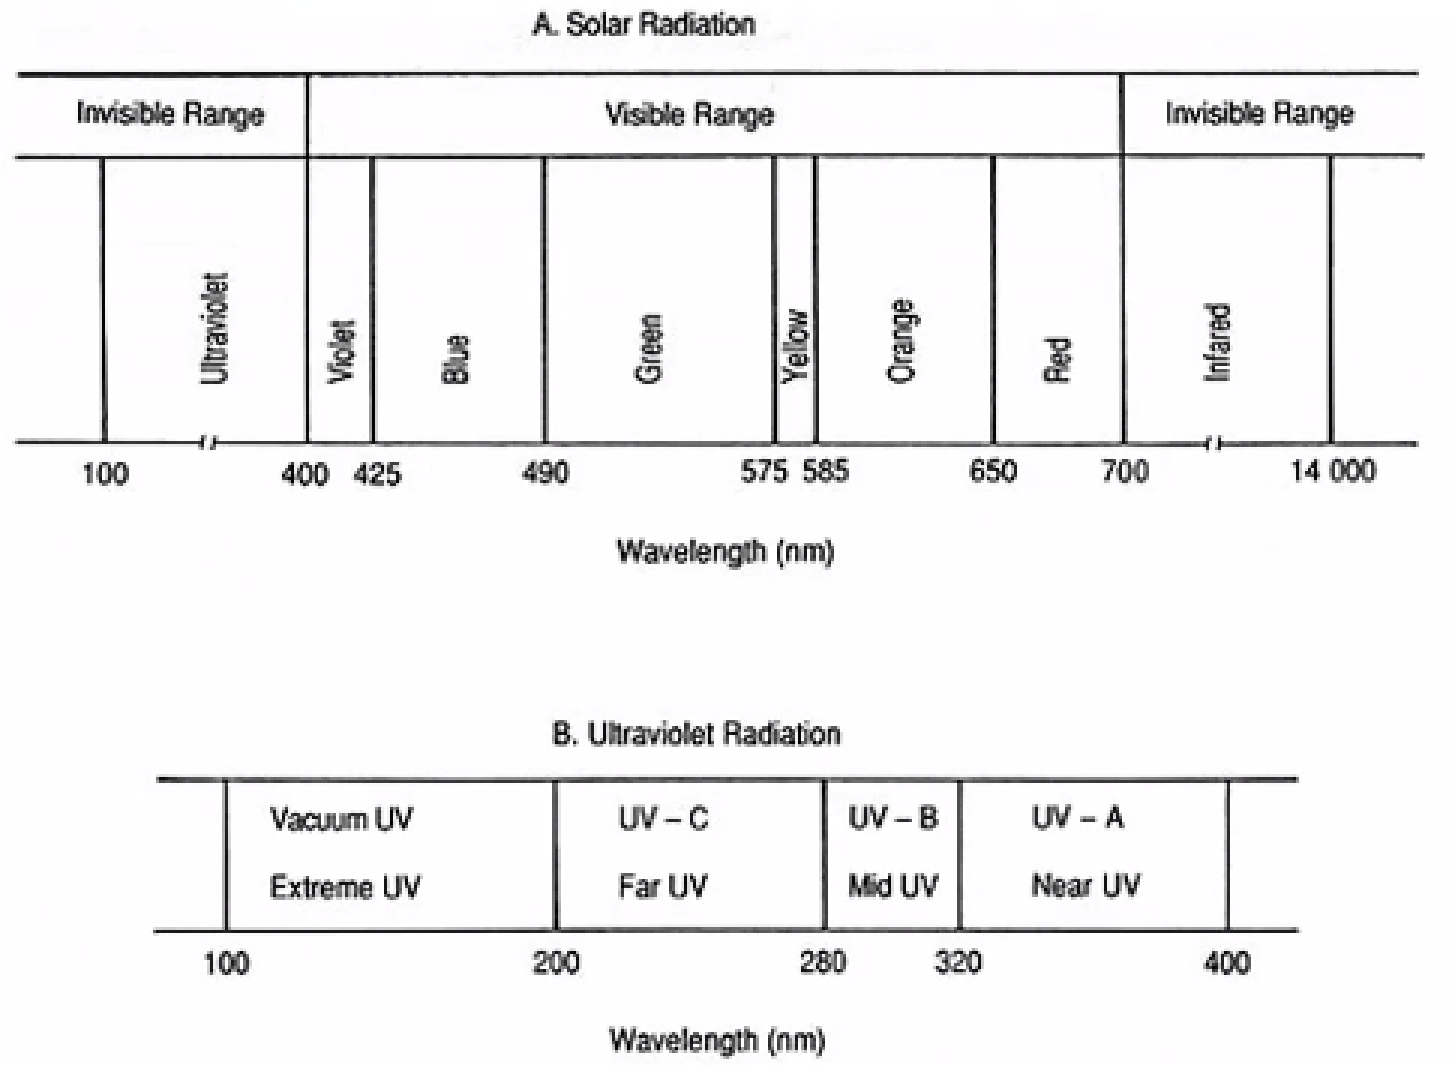
\includegraphics[width=0.5\textwidth]{t1.png}}
  \caption{Radiación solar y longitud de onda}
  \label{t1}
\end{figure}

\subsubsection{Difracción de Rayleigh}
Cuando la radiación cae a una superficie, refleja la longitud de onda $\lambda$ se descompone con una longitud de onda diferente hacia todas partes. Provocada por las partículas de polvo y moléculas de gases atmosféricos (como $N_2$ y $O_2$) con diámetros menores que la onda de la radiación que incide en ellas.

Es mayor para las longitudes de onda del azul y el UV. Es responsable de ambos colores azul del cielo y de los colores rojos brillantes y anaranjado de la puesta del sol.\footnote{La luz azul es difractada cuatro veces más que la luz roja, y la luz UV casi 16 veces que la luz roja}

\begin{figure}[h!]
  \centerline{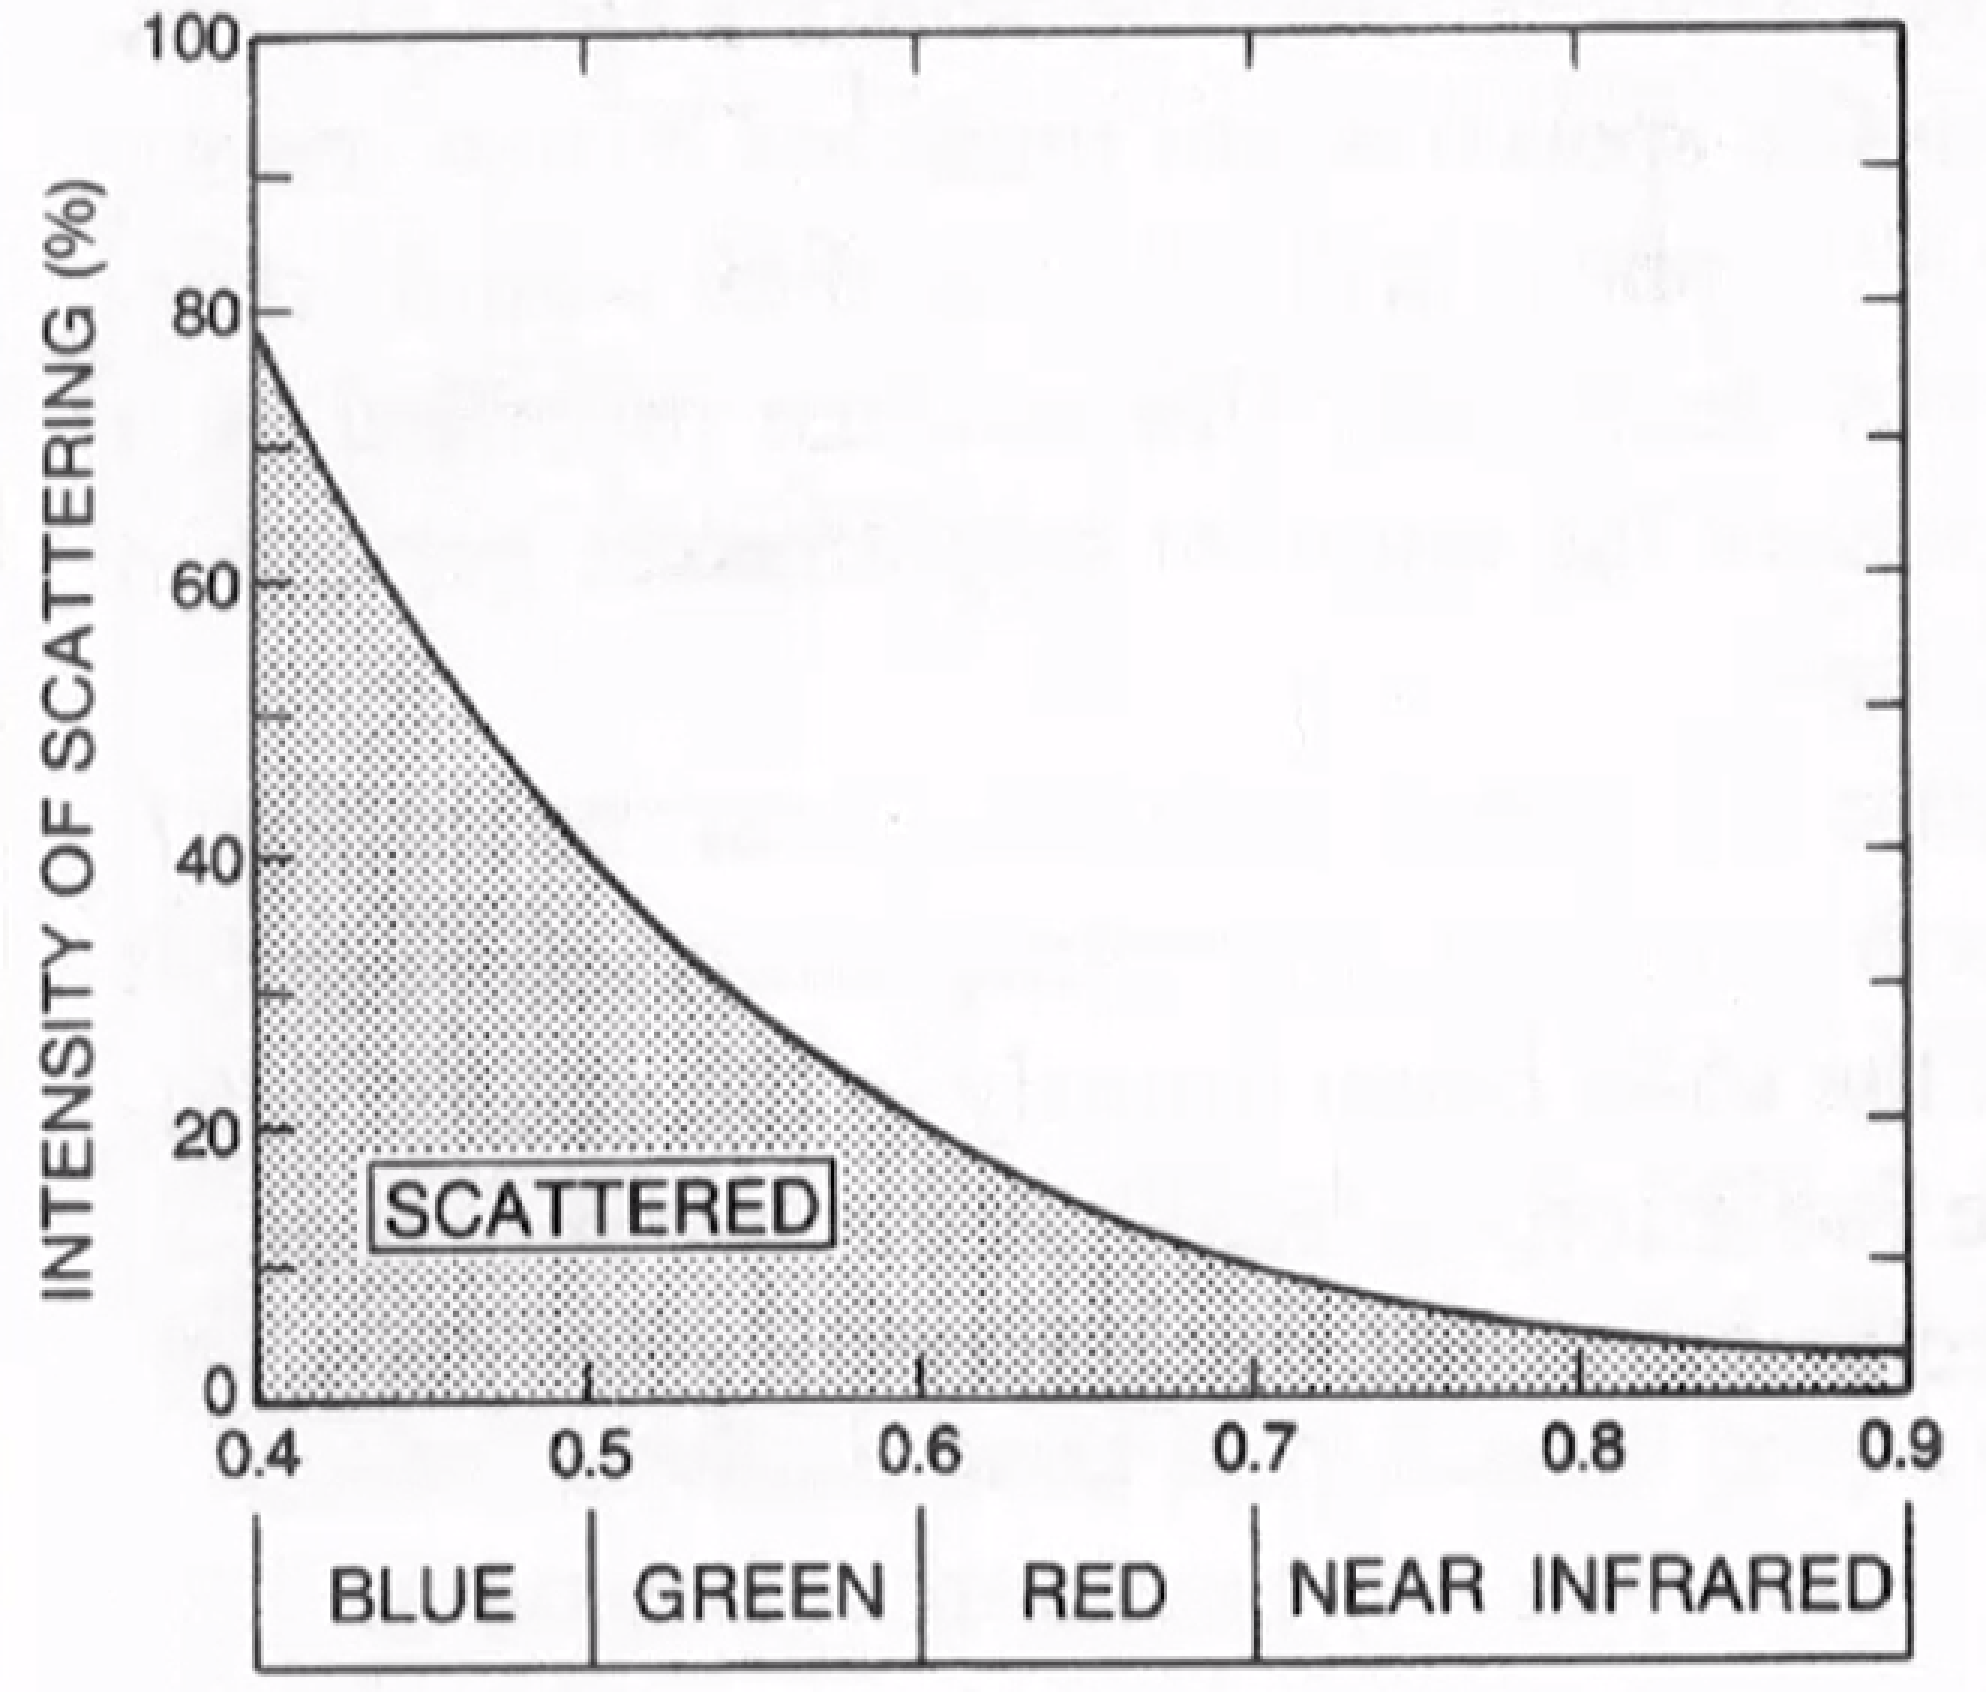
\includegraphics[width=0.5\textwidth]{t2.png}}
  \caption{Difracción de Rayleigh}
  \label{t2}
\end{figure}

\subsubsection{Difracción de Mie}

Ocurre cuando el tamaño de las partículas es comparable a la longitud de onda de la radiación que incide en ellas

La difracción de Mie se manifiesta como una deterioración general de las imágenes multiespectrales cuando estas fueron registradas bajo neblinas pasadas.

\subsubsection{Difracción non selectiva}

Ocurre cuando el tamaño de las partículas difractantes es mayor que la longitud de onda de la radiación incidente. Cuando la atmósfera está cargada de polvos

\subsection{Sensores}

\begin{figure}[h!]
  \centerline{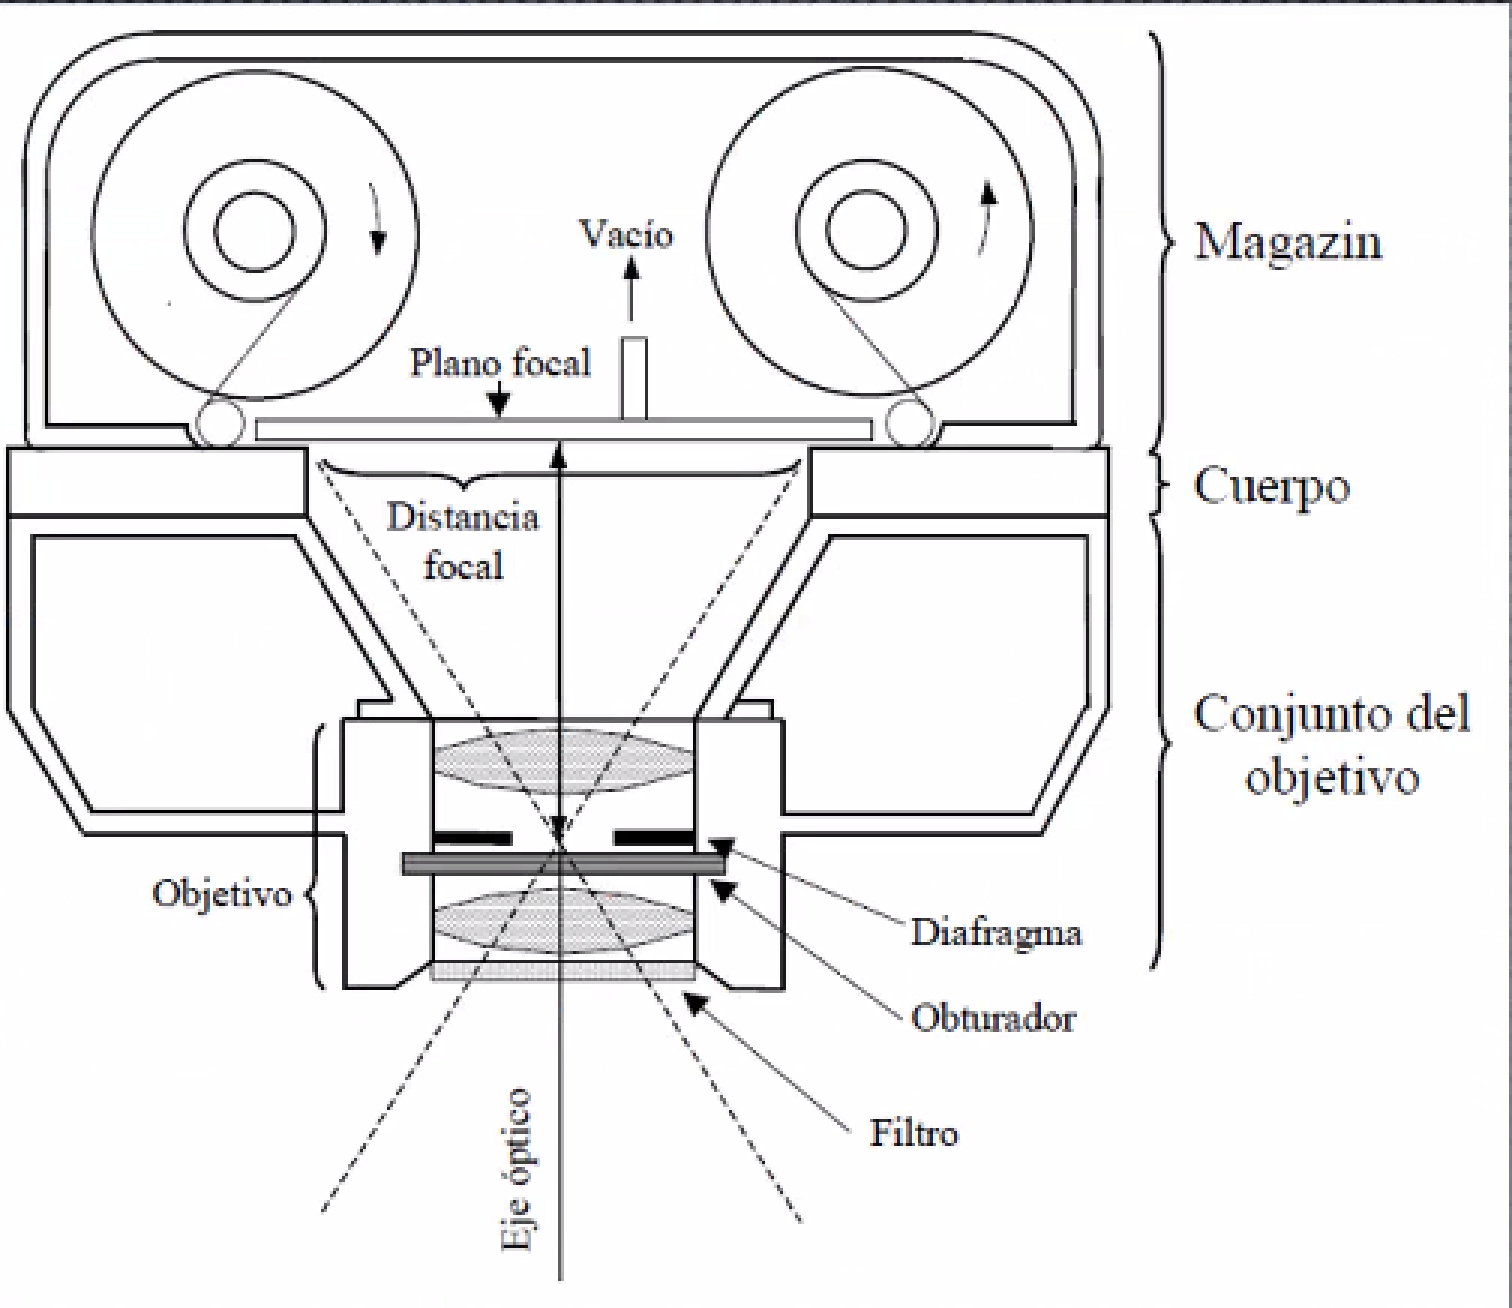
\includegraphics[width=0.5\textwidth]{t3.png}}
  \caption{Cámara de visión}
  \label{t3}
\end{figure}


\begin{table}[h!]
  \centering\begin{tabular}{@{}cccc@{}}
    \toprule
    Tipo de cámara     & Ángulo de abertura & Distancia focal & Características y uso                                                                      \\ \midrule
    Ángulo normal      & $75^{\circ}$                & 300mm           & \begin{tabular}[c]{@{}c@{}}Menor distorsión radical\\ y mayor altura de vuelo\end{tabular} \\
    Gran angular       & $88^{\circ}$                & 150mm           & \begin{tabular}[c]{@{}c@{}}Escalas medias y\\ grandes de cartografía\end{tabular}          \\
    Super gran angular & $150^{\circ}$               & 88mm            & \begin{tabular}[c]{@{}c@{}}Mayor distorsión radial.\\ Escalas pequeñas\end{tabular}        \\ \bottomrule
    \end{tabular}
    \caption{Tipo de cámaras }
    \label{tabt1}
    \end{table}

\subsubsection{Tipo de Fotografía aérea}

Existe la fotografía vertical, fotografía Oblicua Baja y fotografía oblicua alta o panorámica, como se muestra en la figura

\begin{figure}[h!]
  \centerline{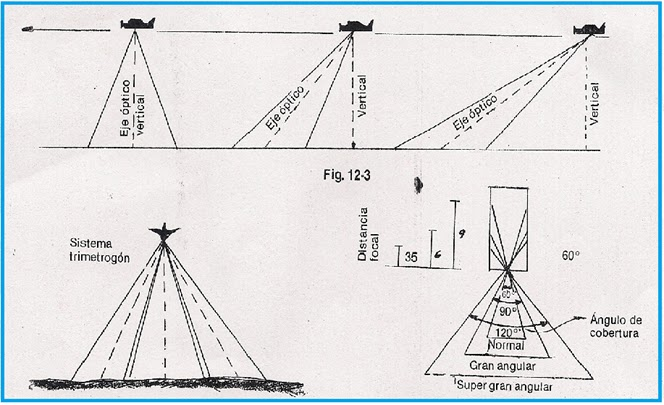
\includegraphics[width=0.5\textwidth]{t4.jpg}}
  \caption{Tipos de fotografía aérea}
  \label{t4}
\end{figure}

\subsubsection{Terminología de las fotografía aéreas}

\begin{figure}[h!]
\centering
\begin{subfigure}[b]{0.45\linewidth}
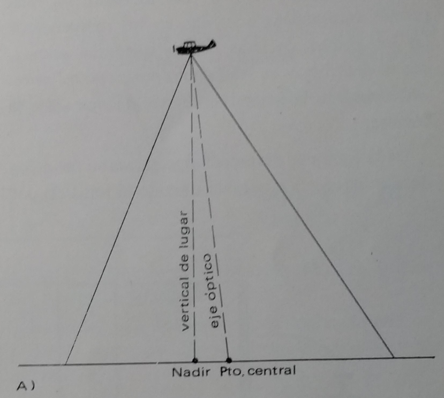
\includegraphics[width=\linewidth]{t5.png}
\caption{Instante 1}
\label{t5}
\end{subfigure}
\begin{subfigure}[b]{0.45\linewidth}
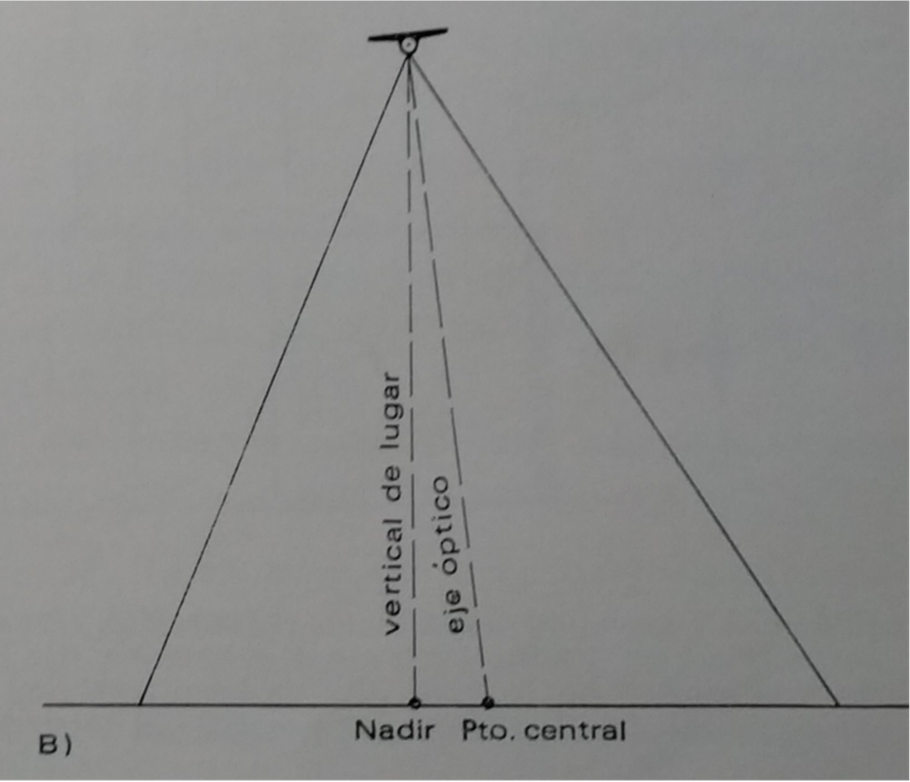
\includegraphics[width=\linewidth]{t6.png}
\caption{instante 2}
\label{t6}
\end{subfigure}
\caption{Solapamiento de fotografías}
\label{t5-6}
\end{figure}

Para obtener las fotografías, es necesario hacer un plan de vuelo,
superposición entre fotos consecutivas: 60\%, también el solapamiento entre bandas de recubrimiento: 25\%

\begin{figure}[h!]
  \centerline{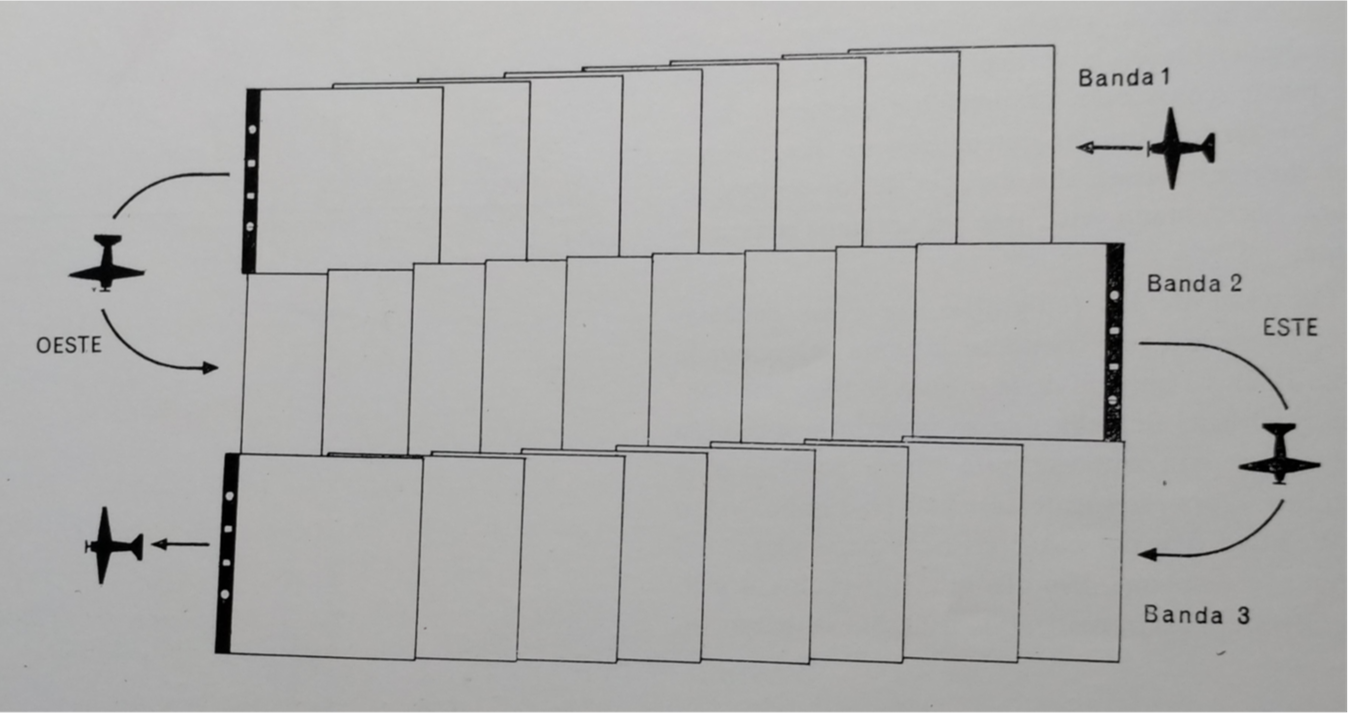
\includegraphics[width=0.5\textwidth]{t7.png}}
  \caption{Plan de vuelo}
  \label{t7}
\end{figure}

\begin{figure}[h!]
  \centerline{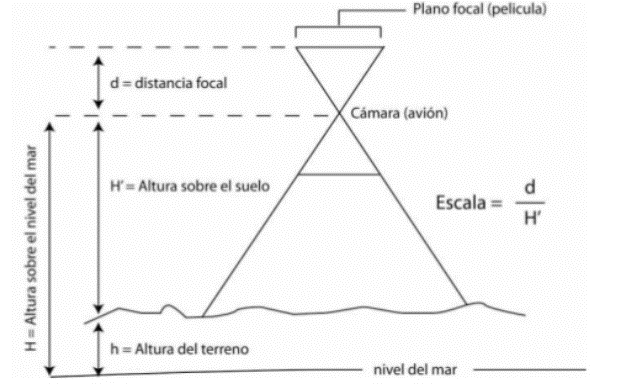
\includegraphics[width=0.5\textwidth]{t8.png}}
  \caption{Escalas de fotografías aéreas}
  \label{t8}
\end{figure}

De los triángulos formados, denotemos AOB y aob como triángulos semejantes, estarían dadas por la relación: 

\begin{equation}
  \frac{1}{E}= \frac{f}{H}=\frac{i}{o}
\end{equation}

\begin{definition}[Desplazamiento]
  En relación con un nivel del terreno, los puntos más altos se alejan del centro de la fotografía, y los puntos más bajos se acercan a este
\end{definition}

EL Desplazamiento aumenta con la altura del objeto y a medida que se incrementa la distancia al centro de la fotografía aéreas 

A medida que aumenta la altura de la cámara, el desplazamiento es menor.                                                                                                               

\begin{figure}[h!]
  \centerline{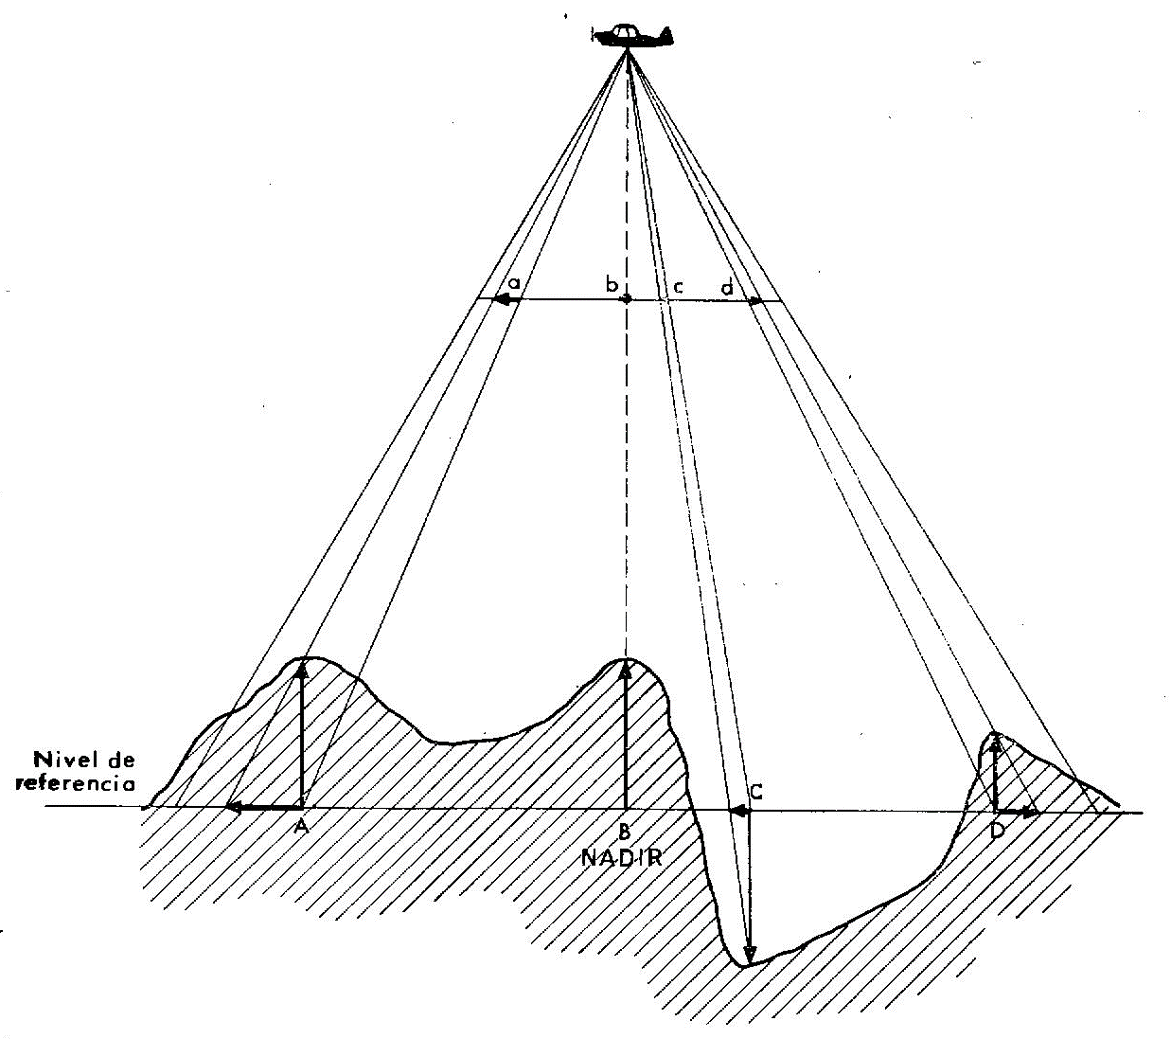
\includegraphics[width=0.5\textwidth]{t9.png}}
  \caption{Escala y desplazamiento de la fotografía aérea}
  \label{t9}
\end{figure}

El desplazamiento causado por la proyección central de un objeto será mayor cuanto mayor sea la distancia de dicho objeto al punto central de la fotografía. 

EL Desplazamiento aumenta con la altura del objeto

A medida que aumenta la altura de la cámara, el desplazamiento es menor

\begin{figure}[h!]
  \centerline{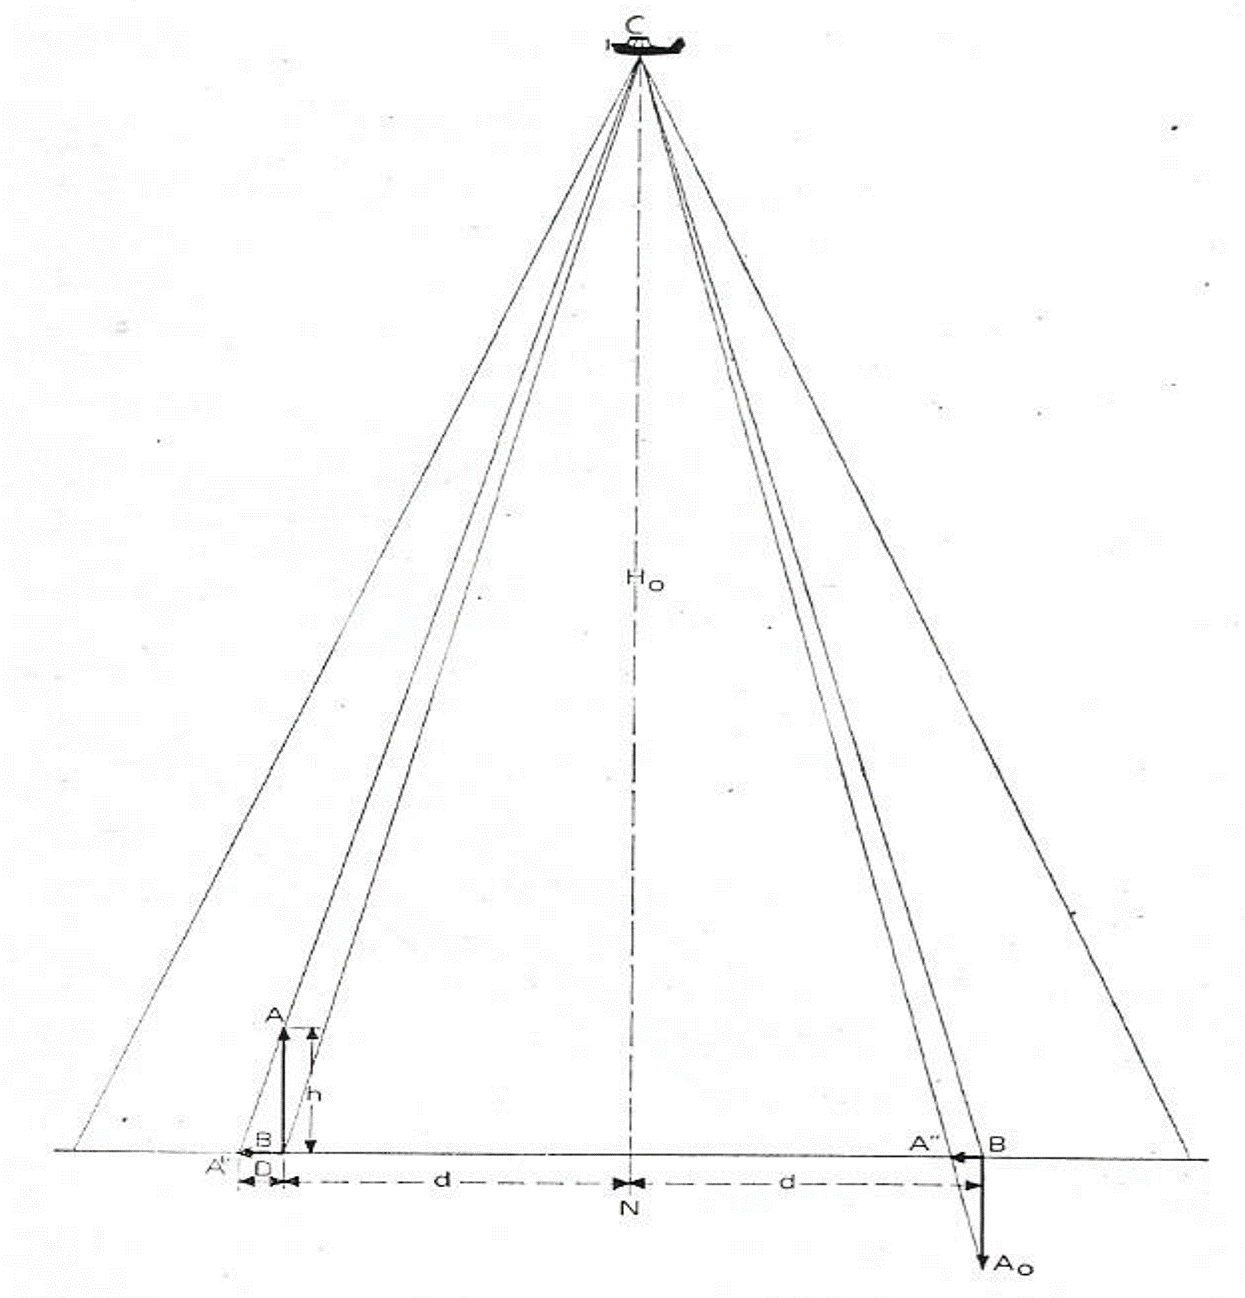
\includegraphics[width=0.5\textwidth]{t10.png}}
  \caption{Punto central de la fotografía}
  \label{t10}
\end{figure}

del fa figura \ref{t10}, podemos deducir las siguientes fórmulas:

\begin{equation}
  D=\frac{h\cdot d}{H_0-h}
\end{equation}

En el caso de estar situado el objeto por debajo del nivel de referencia, que en este caso sería $A_0B$, la semejanza la estableceremos entre los triángulos $a^{\prime\prime}CN$ y $A^{\prime\prime} A_oB$

En los casos en que la altura del objeto sea despreciable frente a la magnitud de la altura de vuelo, la fórmula puede quedar reducida a: 
\begin{equation}
  D=\frac{h\cdot d}{H_o}
\end{equation}
Siendo $D$ el desplazamiento, $H_o$ la altura de vuelo sobre el terreno, $h$ la altura del objeto, $d$ distancia del Nadir a la base del objeto.

Se puede medir la altura de los objetos en las fotos aéreas midiendo el desplazamiento con la siguiente fórmula:

\begin{equation}
  h=\frac{H_0\cdot D}{d+D}
\end{equation}

\subsubsection{Visión estereoscópica}

La visión en relieve se logra en la vida real por la visión simultánea de los objetos desde distintos ángulos, el correspondiente a cada ojo, y su coordinación mental. Gracias a esta doble visión, podemos apreciar las distancias, espesores, profundidades, es decir todas aquellas magnitudes tridimensionales de los objetos

Las dos fotografías descritas reciben el nombre de par estereoscópico, y en el caso de las fotografías verticales pueden ser cualquier par de fotografías consecutivas a lo largo de una línea de vuelo, siempre que cumplan los siguientes requisitos:

\begin{enumerate}
  \item Deben ser de una escala igual o muy aproximada, si hay grandes desniveles de terreno o ha variado la altura del avión, la visión se dificulta pudiendo llegar a impedirse.
  \item El solapamiento de las fotografías debe ser de un 60 por 100 del terreno fotografiado óptimo
  \item El rumbo del avión debe ser constante para que una foto no quede girada con respecto a la otra
  \item La verticalidad de la cámara en el momento de la exposición debe ser menor de $2^{\circ}$.
\end{enumerate}


\begin{definition}[Estereoscopios]
  Son aparatos de los cuales nos servimos para coordinar mentalmente dos fotografías de un mismo objeto, tomadas desde distinto ángulo de manera que logramos una imágen virtual tridimensional del mismo. Véase la figura \ref{t11}
\end{definition}

\begin{figure}[h!]
  \centerline{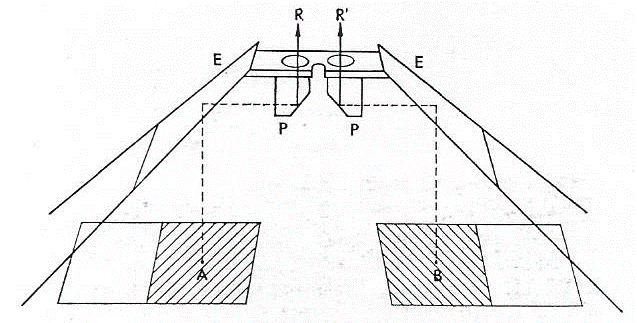
\includegraphics[width=0.5\textwidth]{t11.png}}
  \caption{Óptica de un estereoscópico}
  \label{t11}
\end{figure}

\begin{definition}[Paralaje]
  También llamado desplazamiento aparente en la posición de un objeto, debido al cambio de punto de observación
\end{definition}

\begin{figure}[h!]
  \centerline{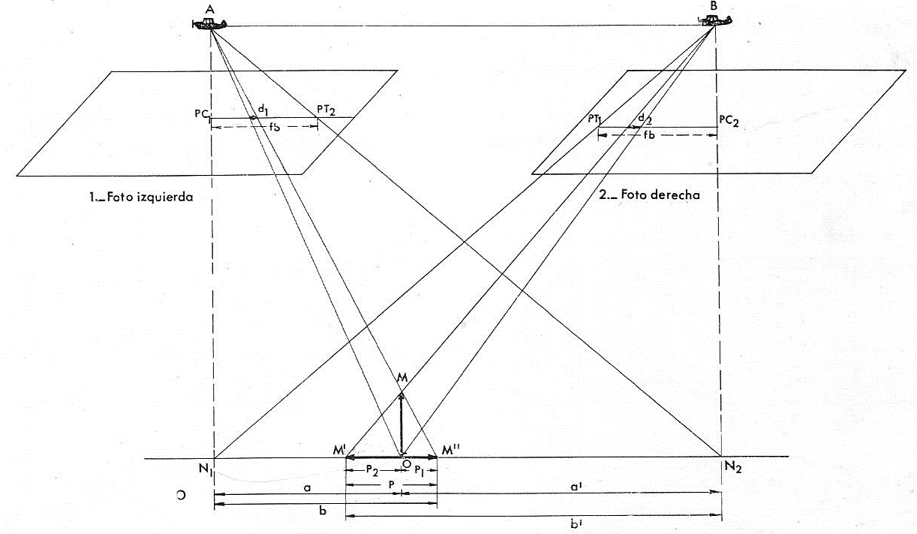
\includegraphics[width=0.5\textwidth]{t12.png}}
  \caption{Muestra la toma de un objeto OM desde dos puntos distintos A y B. Desde el punto $A$, la punta de la flecha se proyectará en $M^{\prime\prime}$, y el desplazamiento $OM^{\prime\prime}$ será el equivalente en la fotografía izquierda a $d_1$ Igualmente, el desplazamiento $OM^{\prime}$, proyección de la flecha OM desde el punto B, queda representado en la fotografía derecha por $d_2$.}
  \label{t12}
\end{figure}

El paralaje absoluto del punto M, punta de la flecha, será $N_1M^{\prime\prime}+N_2M^{\prime}$. El paralaje del punto O, base de la flecha $N_1O+N_2O$. La diferencia de paralaje entre el punto $M$ y el $O$ será 

\begin{equation*}
  \left(N_1M^{\prime\prime}+N_2M^{\prime}\right)-\left(N_1O+N_2O\right)=\left(N_1M^{\prime\prime}-N_1O\right)+\left(N_2M^{\prime}-N_2O\right)\implies
\end{equation*}
\begin{equation}
  P=P_1+P_2
\end{equation}

El paralaje es directamente proporcional a la altura del punto. Se considera el eje $x$ la línea de vuelo con signo + según la dirección de vuelo, se puede usar para determinar alturas en las fotos aéreas.

\begin{figure}[h!]
  \centerline{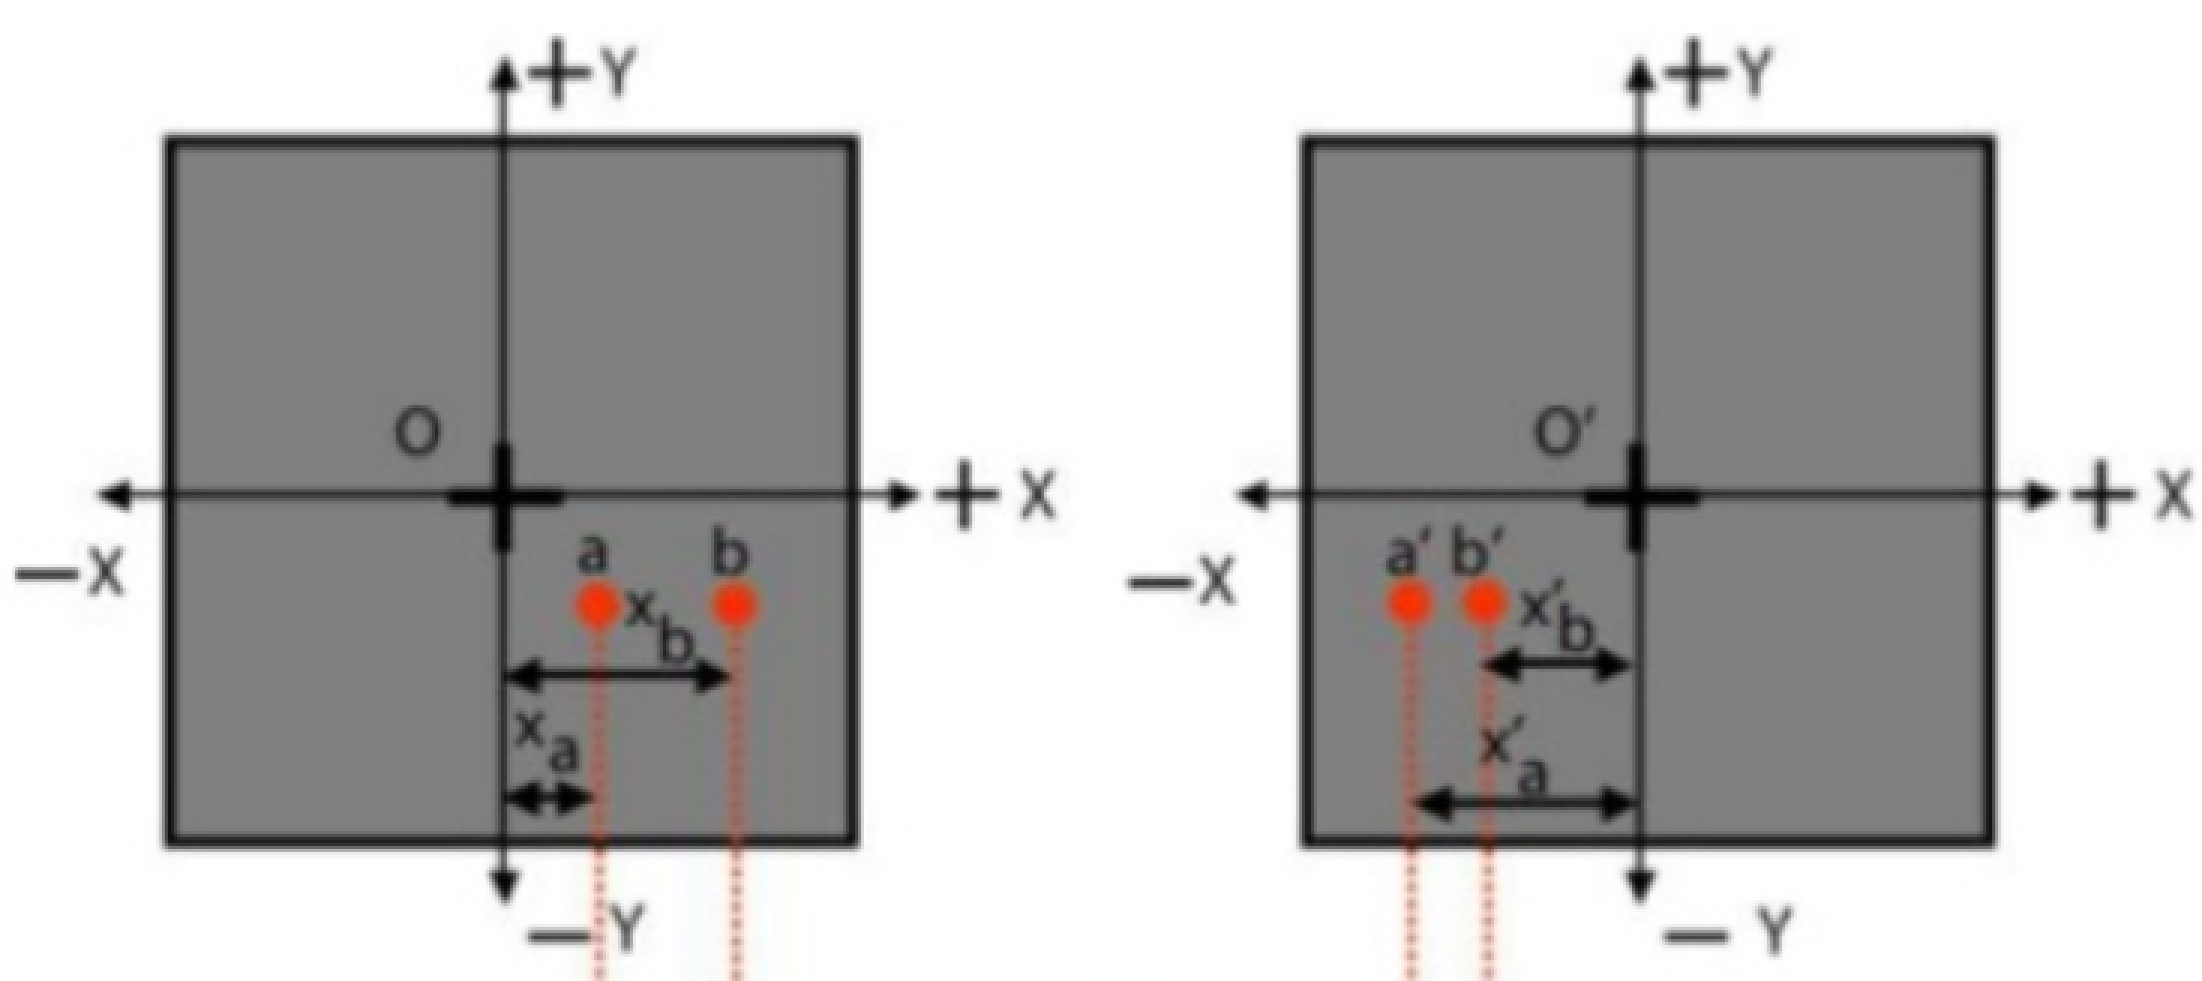
\includegraphics[width=0.5\textwidth]{t13.png}}
  \caption{Barra de baralaje}
  \label{t13}
\end{figure}
\begin{align*}
  &P_a=x-x^{\prime}\\
  &P_a=54.61-(-59.45)=114.06mm\\
  &P_b=x-x^{\prime}\\
  &P_b=98.67-(-27.39)\\
  &\Delta P=12.00
\end{align*}

Se llama paralaje absoluto de un punto en un par estereoscópico de fotografías, a la suma algebráica de la distancia que existe entre la imágen de dicho punto en cada fotografía y los puntos centrales de cada una. Esta distancia debe ser medida paralela a la línea de vuelo

\subsection{Fotointerpretación}

Información geológica que se puede obtener de fotos aéreas:
\begin{itemize}
  \item Litologías
  \item Estructuras
\end{itemize}
La información que podremos obtener dependerá fundamentalmente:
\begin{itemize}
  \item Tipo de clima
  \item Tipo de terreno
  \item Estado de relieve en ciclo geomorfológico
\end{itemize}

\begin{table}[h!]
  \centering\begin{tabular}{|c|c|c|}
  \hline
  Clima                   & Color y reflectividad   & Grado de erosión   \\ \hline
  Cobertura de vegetación & Estructuras geológicas  & Alteración química \\ \hline
  Desarrollo de suelos    & Características físicas & Más elementos      \\ \hline
  \end{tabular}
  \caption{Factores que afectarán a la apariencia de las distintas litologías en las fotos.}
  \label{tabt2}
  \end{table}

%\textbf{De tono blanco a gris claro:}
%
%Nieve, agua reflejando luz, nubes, olas, evaporitas, caliche, barreal, ciertas arenas y gravas, dunas, rasgos de alteración hidrotermal (talco, amianto), corales, cuerpos, cuarzo-del despáticos, diques ácidos, pegmatitas, cuarcitas y calizas
%
%\textbf{Tono gris mediano:}
%
%Yeso, rocas calcáreas y dolomíticas, areniscas claras, arcillitas, lutitas, limolitas, margas, intrusivas y efusivas leucocráticas y básicas
%
%\textbf{De tono gris oscuro a negro}
%DIAPOSITIVA 51
%Sombra de lagos y cursos de agua, césped, carbón, areniscas y lutitas rojas, grauvacas oscuras, areniscas con contenido orgánico, rocas intrusivas, efusivas, básicas y ultrabásicas

El tono está determinado en muchos casos por el contenido de agua, humedad y permeabilidad de la roca, y consecuentemente por la vegetación. La selección del filtro puede en algunos casos separar efectivamente dos rocas de diferente litología, aunque aparentemente similares en fotos tomadas sin filtro. Dependiendo de los elementos que causan el cambio de tono, la textura puede tener un aspecto grueso, fino, uniforme, liso, lineado, moteado o bandeado.
\begin{itemize}
  \item Textura geomorfológica se refiere al grado de disección del relieve, a la densidad del drenaje y la frecuencia de los cursos de agua en un área determinada.
  \item Textura litológica el cambio de tono se debe a una distinta composición mineralógica o a meteorización, rasgos acentuados por un notable bandeado, particularmente evidente en ambientes áridos
  \item Textura de erosión, se refiere al aspecto fino o grueso de la roca; son de tono relativamente más claro y ``textura de erosión'' uniforme y fina las rocas con superficies lisas, por ejemplo las lutitas; las rocas fracturadas como las graníticas o material de grano grueso como conglomerados, presentan una textura de erosión gruesa y poco uniforme.
\end{itemize}

También son de tono relativamente más claro, rocas desteñidas o descoloridas, áreas cubiertas por vegetación caduca, y en zonas situadas en clima árido. Además en ambientes húmedos, las pendientes expuestas al sol pueden soportar una vegetación más densa y resultar con un tono más oscuro que en ambientes áridos, donde las partes expuestas al sol son secas y se caracterizan por un tono más claro.

\subsubsection{Textura}
Es el modo de presentarse, en conjunto, de un agregado de rasgos individuales bastante pequeños para ser distinguidos en forma individual. Es muy importante tener en cuenta la escala.

\begin{itemize}
  \item Ser toscas o finas
  \item Ásperas o suaves
  \item Uniformes o desiguales
  \item Punteadas, rayadas, granulares, esponjosas, jaspeadas.
\end{itemize}
La textura depende de:
\begin{enumerate}
  \item \textbf{Clima:} Como las calizas cavernosas, tan peculiares de las zonas tropicales, la tienen tan marcada, que son fáciles de localizar en cualquier parte, simplemente por su textura.
  \item \textbf{Escala:} Una textura fina o suave, en una fotografía aérea hecha a pequeña escala, se convertirá en una textura gruesa o áspera, en una fotografía hecha a gran escala.
\end{enumerate}

\subsubsection{Forma y tamaño}

La forma y el tamaño relacionados con la escala son los factores que ayudan al foto interprete a identificar los rasgos geológicos, dado que estos rasgos están íntimamente relacionados con la forma del relieve terrestre. La erosión diferencial proporciona valiosos criterios para identificar estructuras rocosas resistentes y no resistentes.

La forma horizontal de los objetos o rasgos es un factor de capital importancia en la identificación de los rasgos u objetos, no sólo en la tarea fotogeológica, sino en cualquier otra que tenga por cometido la identificación de los mismos.

\subsubsection{Sombra}

Este factor depende de las condiciones de iluminación y tiene que ser tomado en cuenta cuando se planea un vuelo con el objetivo de reducir los efectos negativos de las sombras. La sombra de hecho puede oscurecer detalles peculiares de los materiales de la superficie

\subsubsection{Patrón de drenaje}

Brinda un indicador muy efectivo de la resistencia del suelo y del material rocoso a la erosión. El drenaje en una zona se encuentra afectado por varios factores, entre los que se encuentran: 

\begin{itemize}
  \item Pendientes iniciales de la superficie del suelo
  \item Estructura de la roca madre
  \item Textura del suelo
  \item Topografía
  \item Vegetación
  \item Clima
  \item Frecuencia e intensidad de las lluvias.
\end{itemize}

Características de las redes de drenaje: 
\begin{itemize}
  \item Integración indica la existencia de conexión entre los cursos de agua de órdenes sucesivos 
  \item La densidad es la cantidad de drenajes superficiales por unidad de superficie.
  \item La orientación no se refiere a un curso o rama en particular, sino al conjunto integrado o no de cursos principales y atributos en una zona
  \item El control estructural se refiere a los cambios bruscos de dirección, que son indicio de modificaciones de las características litológiacas o morfológicas del subsuelo
  \item La forma de la red viene supeditada a la estructura de las rocas.
\end{itemize}

\section{Fundamentos de la percepción remota}

La Percepción Remota es una actividad muy familiar que realizamos  cada día. La luz que emana de un  objeto ubicado a cierta distancia (remota) llega a nuestro ojo que es el censor. 

Cada ojo envía una señal al procesador que es nuestro cerebro, este último almacena los datos y los interpreta en información. 
        El modo de operación de los otros sentidos del hombre, en particular el sentido del oído que registra las ondas del sonido, opera de igual modo.
 
En la práctica, nunca nos imaginamos que nuestros sentidos funcionan como sensores remotos

La Percepción Remota es el término usualmente empleado para el 
estudio de los objetos remotos (tierra, luna, superficies planetarias y atmósfera, fenómenos estelares y galácticos, etc.)

La percepción Remota implica el uso de sensores modernos, equipos de procesamiento de datos, metodología de procesamiento y teoría de la información y de la comunicación, los instrumentos, vehículos espaciales (National Academy of sciences, 1970, p.1)

En Percepción Remota la imagen es obtenida con un sensor, no con  
una cámara convencional, usando radiación electromagnética que va 
más allá  del rango visual normal de la película fotográfica de la cámara

\begin{definition}[percepción remota ]
  La colección y medición de datos / información acerca de algunas propiedades de un fenómeno, objeto, o material usando un instrumento sin estar en contacto físico directo con los elementos mencionados.
\end{definition}

Las técnicas consisten en generar conocimientos a cerca del medio físico midiendo los campos de fuerzas, la radiación electromagnética, o energía acústica usando cámaras, radiómetros y escáneres, láser, receptores de frecuencia de radio, sistemas de radar, sondas, instrumentos termales, sismógrafos, magnetómetros, gravímetros, y otros instrumentos. 

Básicamente, la Percepción Remota es el arte o ciencia de hablar acerca de un objeto sin estar en contacto con él (Fisher et al. 1976, p. 34). 

Lintz y Simonett (1976, p. 1) definen la Percepción Remota como la adquisición de datos físicos de un objeto sin tocarlo o estar en contacto con él.

La percepción remota es la observación de un objeto con un instrumento  separado de él por cierta distancia (Barrett \& Curtis, 1996, p3).

En su significado más general, la percepción remota significa, “Reconocimiento a distancia.”(Colwell, 1966, p.71).

\subsection{Sensores}
De acuerdo con el número de bandas:
\begin{itemize}
  \item Pancromático
  \item Multiespectral 
  \item Hyperspectral, y
  \item Ultra espectral sensores
\end{itemize}
De acuerdo al tipo de detector
\begin{itemize}
  \item Detectores termales
  \item Detectores de fotones
\end{itemize}
De acuerdo al modo de escaneo
\begin{itemize}
  \item Detectores Whiskbroom   
  \item Detectores Pushbroom
\end{itemize}

\begin{figure}[h!]
  \centering
  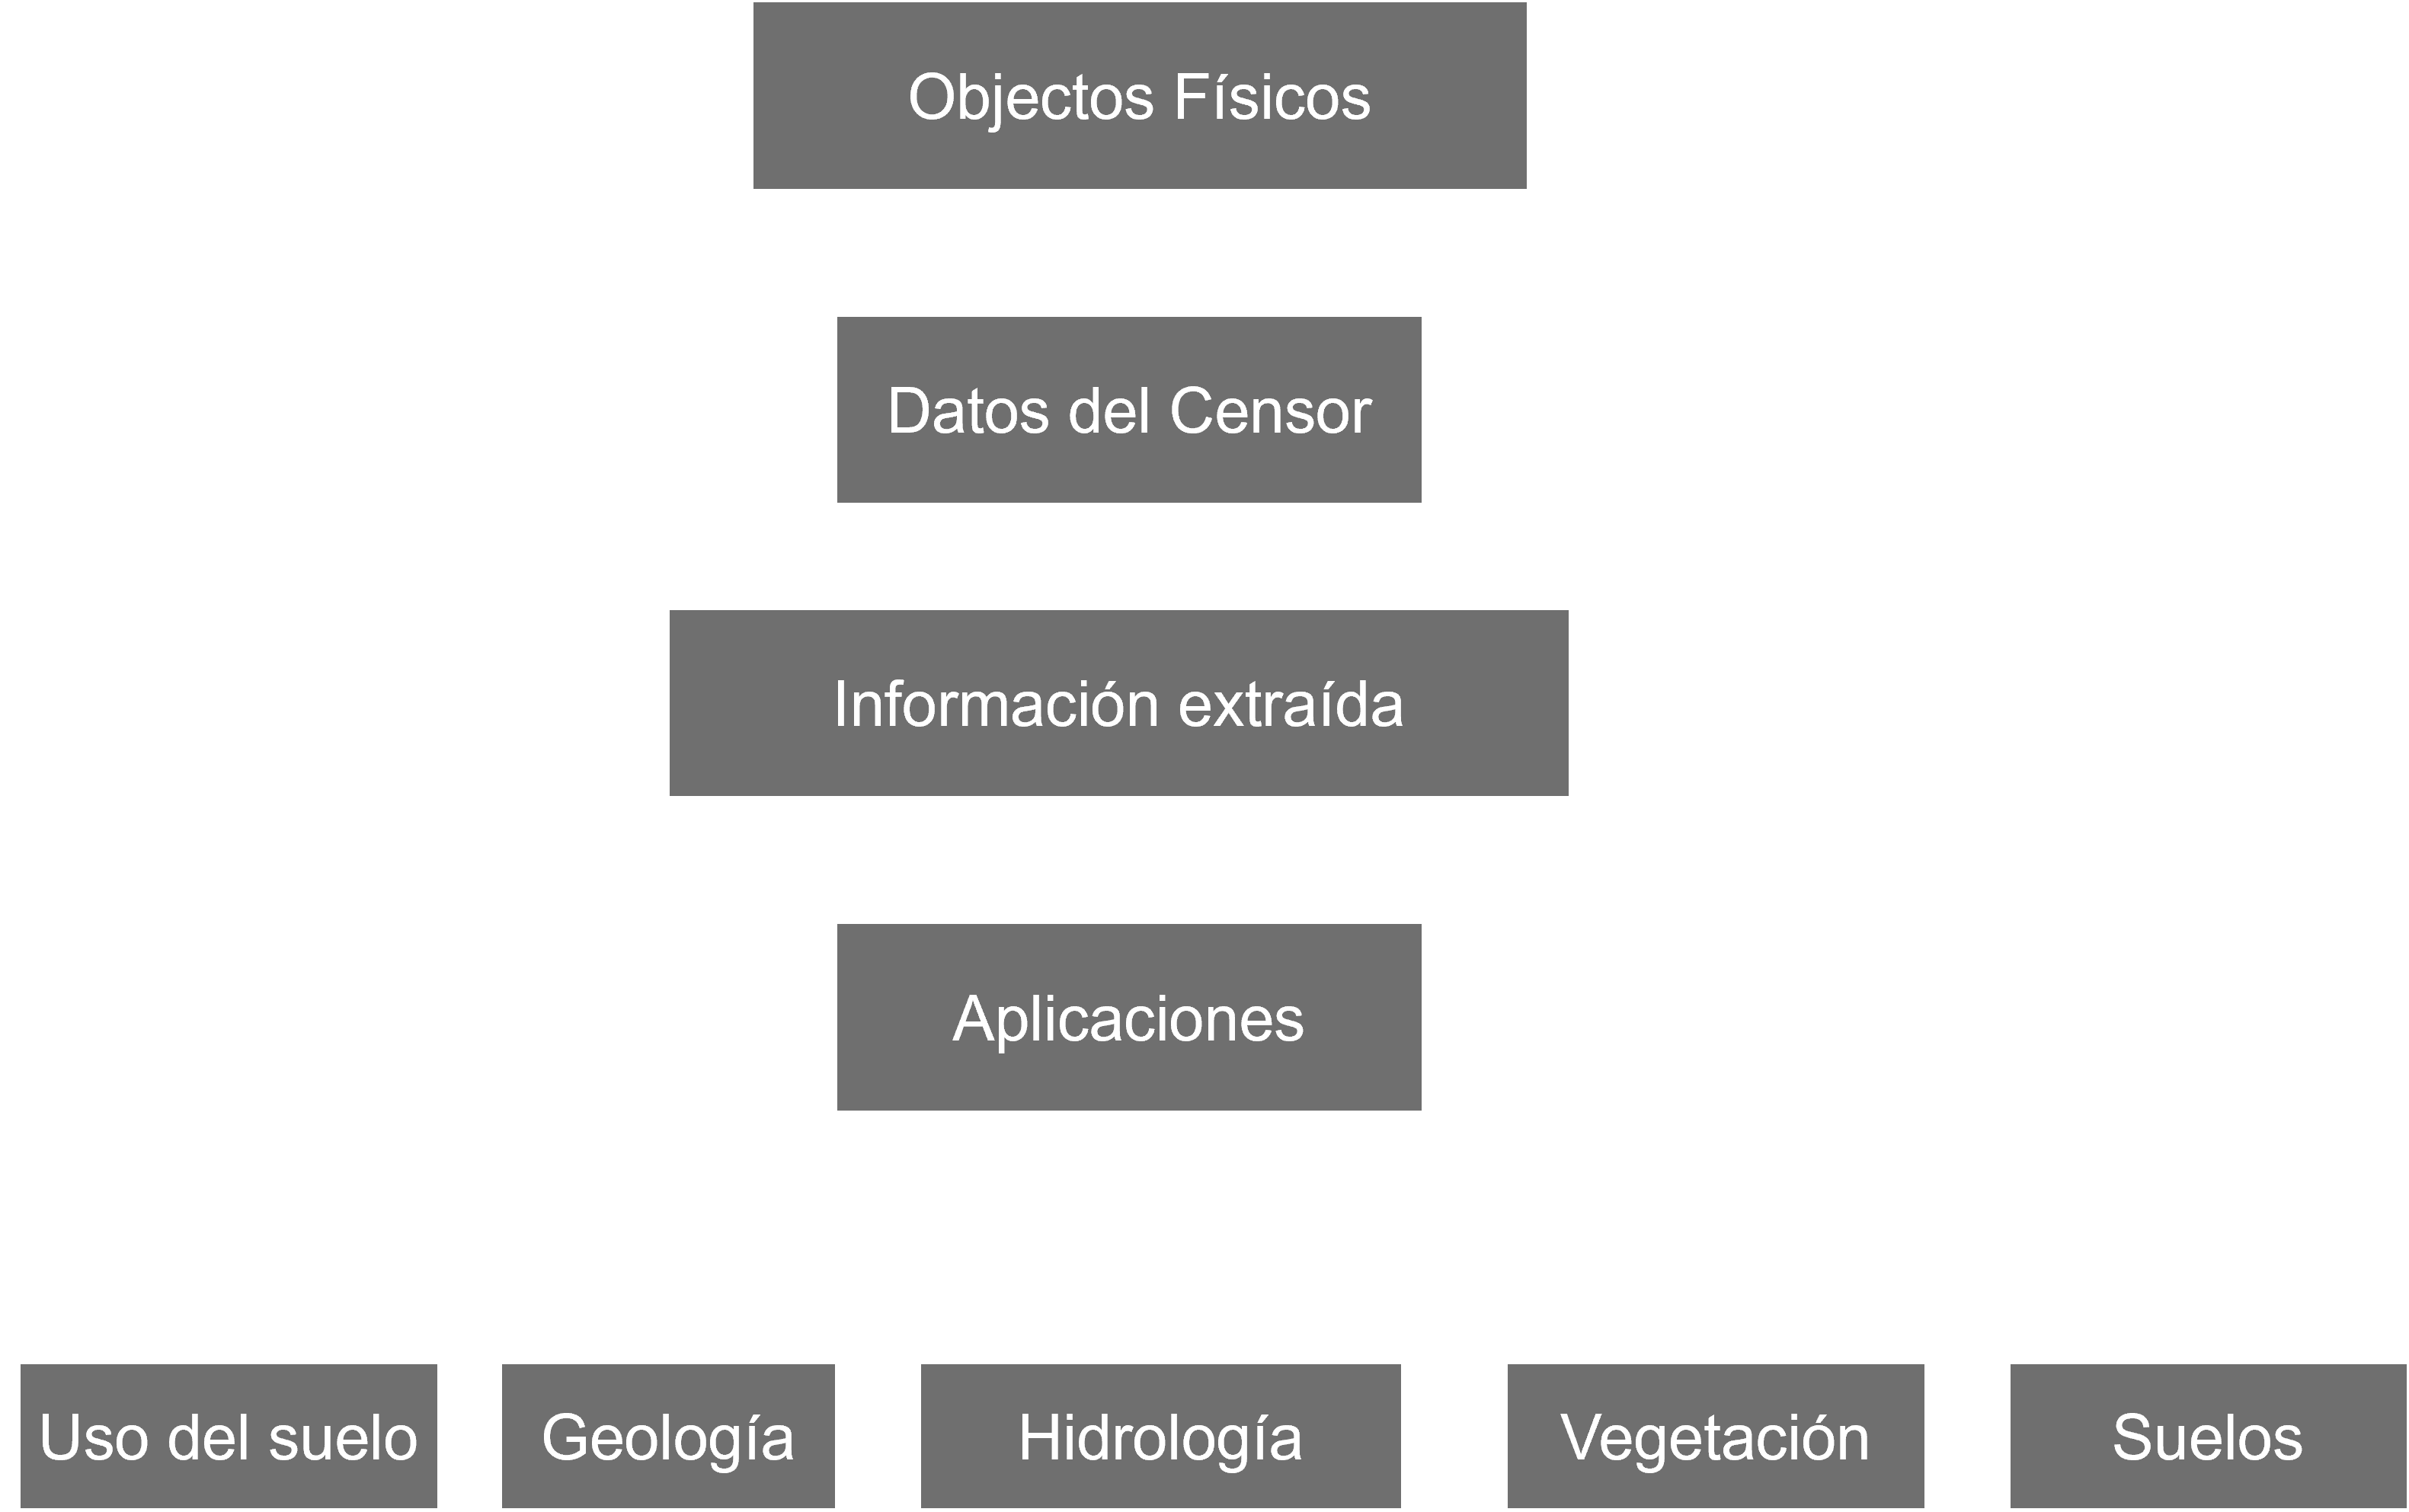
\includegraphics[width=0.5\textwidth]{t15.png}
  \caption{Procesos de la percepción remota}
  \label{t15}
\end{figure}

\begin{figure}[h!]
  \centerline{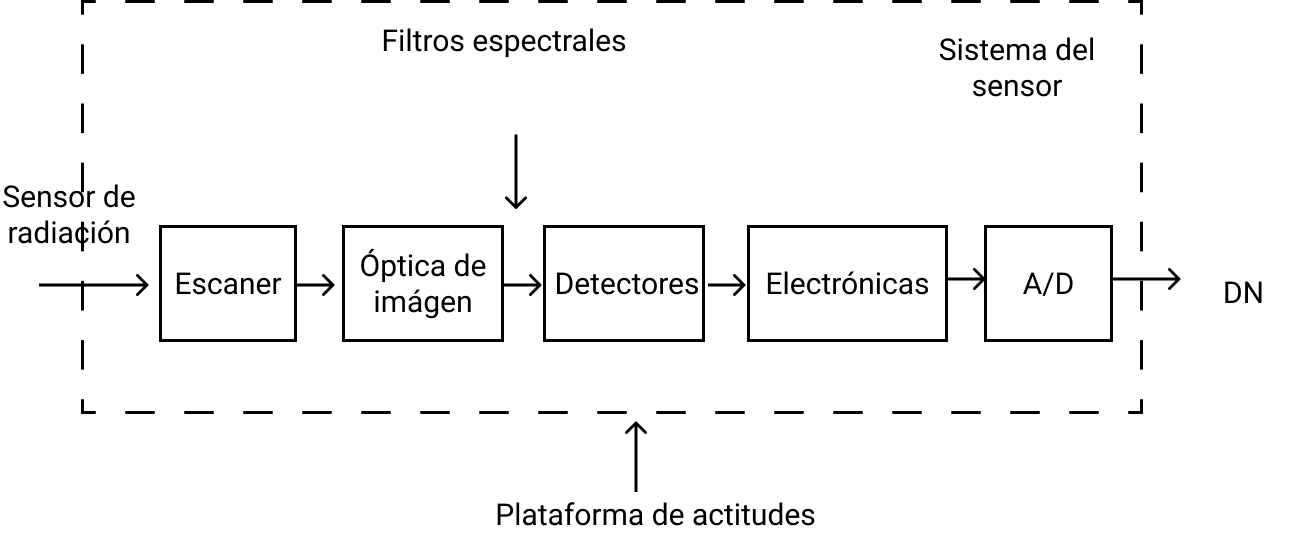
\includegraphics[width=0.5\textwidth]{t14.png}}
  \caption{Los componentes primarios en un sistema óptico-electro sensor remoto}
  \label{t14}
\end{figure}
De acuerdo con el número de bandas
\begin{itemize}
  \item Pancromátrico
  \item Multiespectral
  \item Hiperespectral
  \item Ultraspectral
\end{itemize}

De acuerdo al tipo de detector:
\begin{itemize}
  \item Detectores termales
  \item Detectores de fotones
\end{itemize}

De acuerdo al modo de escaneo
\begin{itemize}
  \item Detectores Whiskbroom
  \item Detectores Pushbroom
\end{itemize}

Sistemas de plataformas de barrido

\begin{itemize}
  \item Sistemas de aeroplanos
  \item Sistemas de satélites
  \item Sistemas terrestres
\end{itemize}

\begin{definition}[Satélites]
  Son vehículos artificiales puestos en órbitas alrededor de la tierra o otros planetas y asteroides, llevan a bordos equipos e instrumentos científicos para realizar tareas definidas. Según el propósito por el cual fueron diseñados, los satélites se clasifican en:
Satélites de comunicaciones (órbitas geosíncronas a 36,000 km)
Satélites terrestres para la observación de la tierra, llevan a bordo sensores terrestres. Son varios y  producen imágenes digitales tales como Landsat, SPOT, WorldView etc. Sus órbitas están entre 700 a 1400 km.
Satélites de geoposicionamiento con órbitas entre 10,000 de 20,500 km de la tierra
Satélites meteorológicos con órbitas geosíncronas.
Etc…
\end{definition}

\begin{itemize}
  \item LANDSAT (LAND = tierra y SAT = satélite) fue el primer satélite enviado por los Estados Unidos para el monitoreo de los recursos terrestres. 
  \item Las imágenes LANDSAT están compuestas por 7 u 8 bandas espectrales, que fueron elegidas especialmente para el monitoreo de la vegetación, para aplicaciones geológicas y para el estudio de los recursos naturales. Estas bandas pueden combinarse produciendo una gama de imágenes de color que incrementan notablemente sus aplicaciones.
\end{itemize}

Sensores:
\begin{enumerate}
  \item Landsat \begin{enumerate}
    \item MSS (Landsat 1, 2, 3)
    \item TM (Landsat 4 y 5)
    \item ETM(+) (Landsat 7)
    \item OLI y TIRS (Landsat 8)
    \item HIPERESPECTRAL 
  \end{enumerate}
  \item SPOT 1, 2, 3, 4, 5, 6, 7
\end{enumerate}

\subsubsection{Sensor TM}

El sensor TM es un avanzado sensor de barrido multiespectral, concebido para proporcionar una mayor resolución espacial, mejor discriminación espectral entre los objetos de la superficie terrestre, mayor fidelidad geométrica y mayor precisión radiométrica en relación con el sensor MSS.

Opera simultáneamente en siete bandas espectrales, siendo tres en el visible, una en el infrarrojo cercano, dos en el infrarrojo medio y una en el infrarrojo termal.

Tiene una resolución espacial de 30 metros en las bandas del visible e infrarrojo medio y 120 metros en la banda del infrarrojo termal.

La escena terrestre registrada por este sensor es de 185 km.

\subsubsection{Sensor ETM}

Landsat- 7,  tiene la capacidad de recolectar, así como transmitir hasta 532 imágenes por día. 

Se encuentra en una órbita Heliosincrónica, que significa que pasa siempre a la misma hora por un determinado lugar. 

Tiene visión de toda la superficie terrestre en un lapso de tiempo de 15 días, y realiza 232 órbitas.

A diferencia de sus antecesores, Landsat 7 posee una capacidad de almacenamiento de 378 gigabytes, equivalente a 100 imágenes. El instrumento esencial a bordo del satélite es el Enhanced Thematic Mapper Plus(ETM+).

Una imagen LANDSAT 7 ETM+ está compuesta por 8 bandas espectrales.

Tiene una banda espectral (Banda Pancromática) con resolución de 15 metros. También, cuenta con características geométricas y radiométricas y una mayor resolución espacial de la banda térmica para 60 m. Estos avances tecnológicos permiten calificar al LANDSAT 7 como el satélite más interesante para la generación de imágenes con aplicaciones directas hasta una escala de 1:25.000, principalmente, en áreas rurales o territorios de grandes extensiones. 

\subsubsection{Sensor OLI}

OLI (Operational Land Imager) utiliza un sensor del tipo "pushbroom" compuesto por una serie de baterías largas de detectores, con más de 7.000 detectores por banda espectral, alineados en su plano focal en su respectivo ancho de banda. El diseño del "pushbroom" lo hace un instrumento más sensible proporcionando una mejor información de la superficie terrestre con menos partes móviles. Sus imágenes tienen una resolución espacial de 49 pies (15 m) pancromáticas y 98 pies (30 metros) (incluido el visible, infrarrojo cercano y el infrarrojo de onda corta) a lo largo de 115 millas (185 kilómetros) de ancho de imagen, cubriendo así amplias zonas de la tierra mientras que proporciona una resolución suficiente como para distinguir las características tales como centros urbanos, granjas, bosques y otros tipos de cubiertas del suelo. 

\subsubsection{Thermal Infrared Sensor (TIRS), }

sensor que mide la temperatura de la superficie terrestre mediante dos bandas del infrarrojo térmico (10 y 11). Gracias a los principios de mecánica cuántica es capaz de distinguir la temperatura de la superficie de la temperatura de la atmósfera. Los datos generados por este sensor tienen una resolución de 100 m y son de gran valor para medir la evapotranspiración y el consumo de agua en la agricultura.

\subsubsection{Sensor hiperespectral}
Cada píxel contiene un espectro continuo que permite su identificación en base a las propiedades de reflectancia del material que lo compone.

\begin{figure}[h!]
\centering
  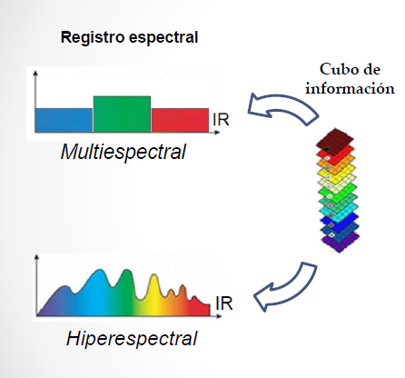
\includegraphics[width=0.5\textwidth]{t16.png}
  \caption{Sensor espectral}
  \label{t16}
\end{figure}

Si bien la mayoría de los sensores hiperespectrales poseen cientos de bandas, no es el número de longitudes de onda observadas lo que define un sensor como hiperespectral, sino que es la continuidad y fineza de sus mediciones. Esto es, la amplitud de la longitud de onda entre cada banda. 

\subsubsection{Firmas espectrales}

El espectro o firma espectral es la medición por un sensor de la luz reflejada por los objetos para cada longitud de onda en un amplio ancho de banda. 
\begin{figure}[h!]
  \centering
    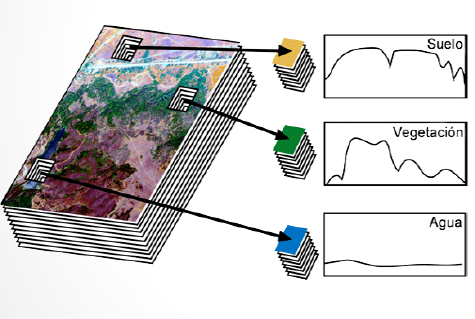
\includegraphics[width=0.5\textwidth]{t17.png}
    \caption{Firmas espectral}
    \label{t17}
  \end{figure}
Cada elemento espacial tiene un espectro continuo que es utilizado para analizar las diversas superficies. 

\section{Introducción al procesamiento digital de imágenes}

\subsection{Estadísticas de las imágenes digitales}

\begin{definition}[Número digital DN]
    Expresa el valor de la intensidad de la luz registrada por los detectores. En una escala de tonos de grises y para una imágen de 8-bit, lEl DN toma valores entre 0 a 255
\end{definition}

\begin{definition}[Dimensional]
    la dimensional de una imágen digital está determinada por el número de bandas $k$
\end{definition}

La Medición del vector $V_k$ de un pixel, es el conjunto de los valores relativos a un pixel en $k$ bandas.
\begin{equation}
    V_K =\begin{bmatrix} 
        v_1\\v_2\\ v_k
     \end{bmatrix}
\end{equation}

\begin{figure}[h!]
\centering
  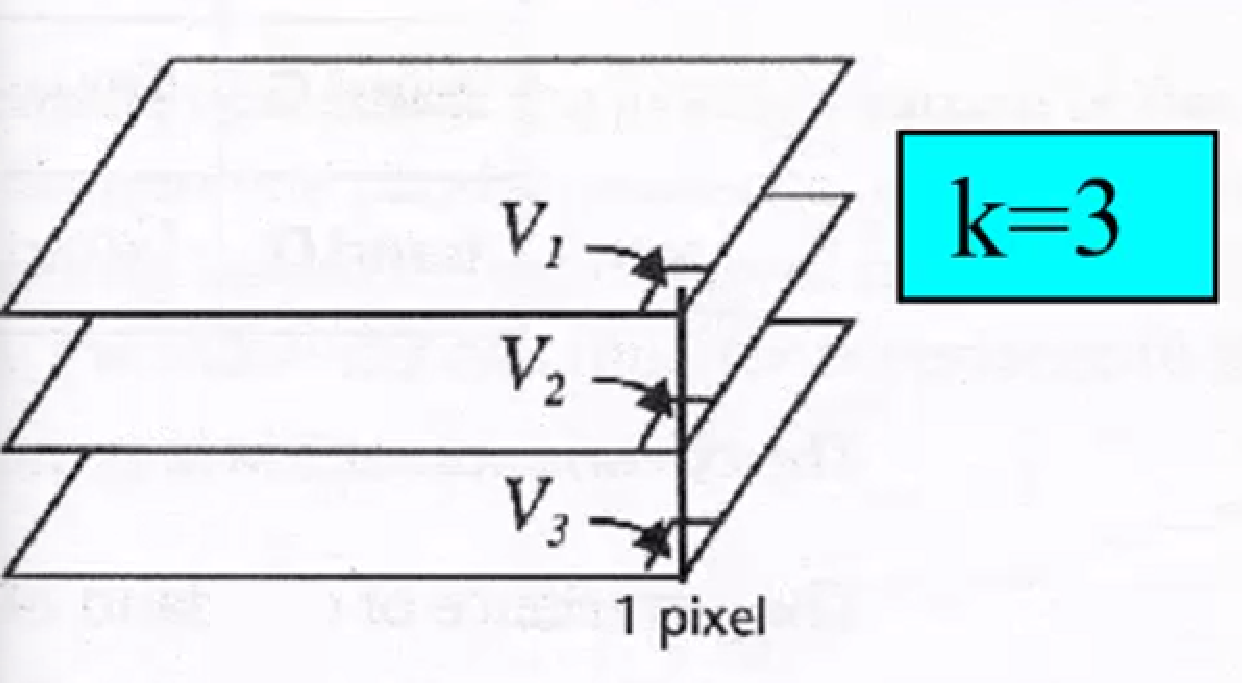
\includegraphics[width=0.5\textwidth]{t18.pdf}
  \caption{Bandas}
  \label{t18}
\end{figure}

Sin embargo, el vector medio, $M_j$ se usa cuando se mide el vector para varios píxeles con la finalidad de representar una clase espectral en $k$ bandas espectrales
\begin{equation}
    M_k =\begin{bmatrix}
        \mu_1\\\mu_2\\\mu_k
    \end{bmatrix}
\end{equation}


\begin{figure}[h!]
    \centering
      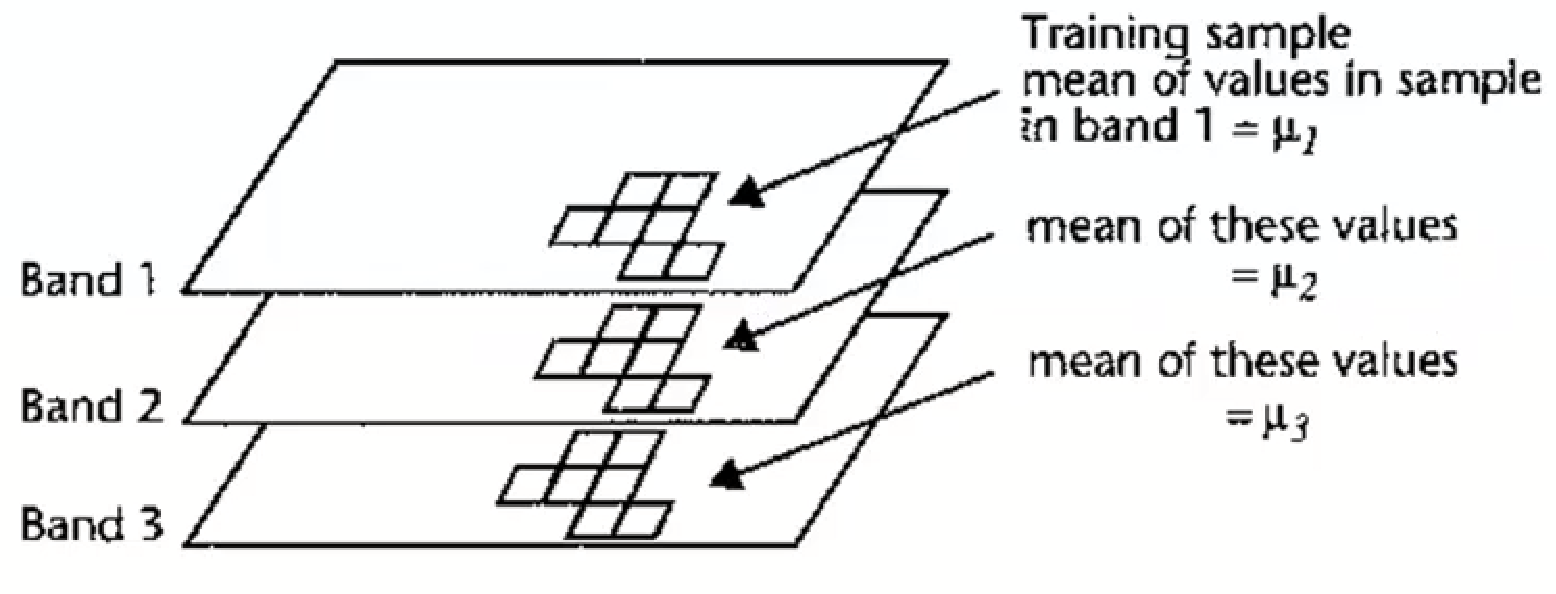
\includegraphics[width=0.5\textwidth]{t19.pdf}
      \caption{Bandas}
      \label{t19}
    \end{figure}

    \begin{notation}
      $i=$ hilera (o línea) en la imágen
      $j=$ columna
      $k=$ el número de bandas espectrales
      $Dn_{i,j,k}=$ El valor de DN en la hilera $i$, la columna $j$ y la banda $k$
  \end{notation}
  \begin{equation}
      Img = bytarr(i,j,k)
  \end{equation}
  
  \begin{figure}[h!]
  \centering
    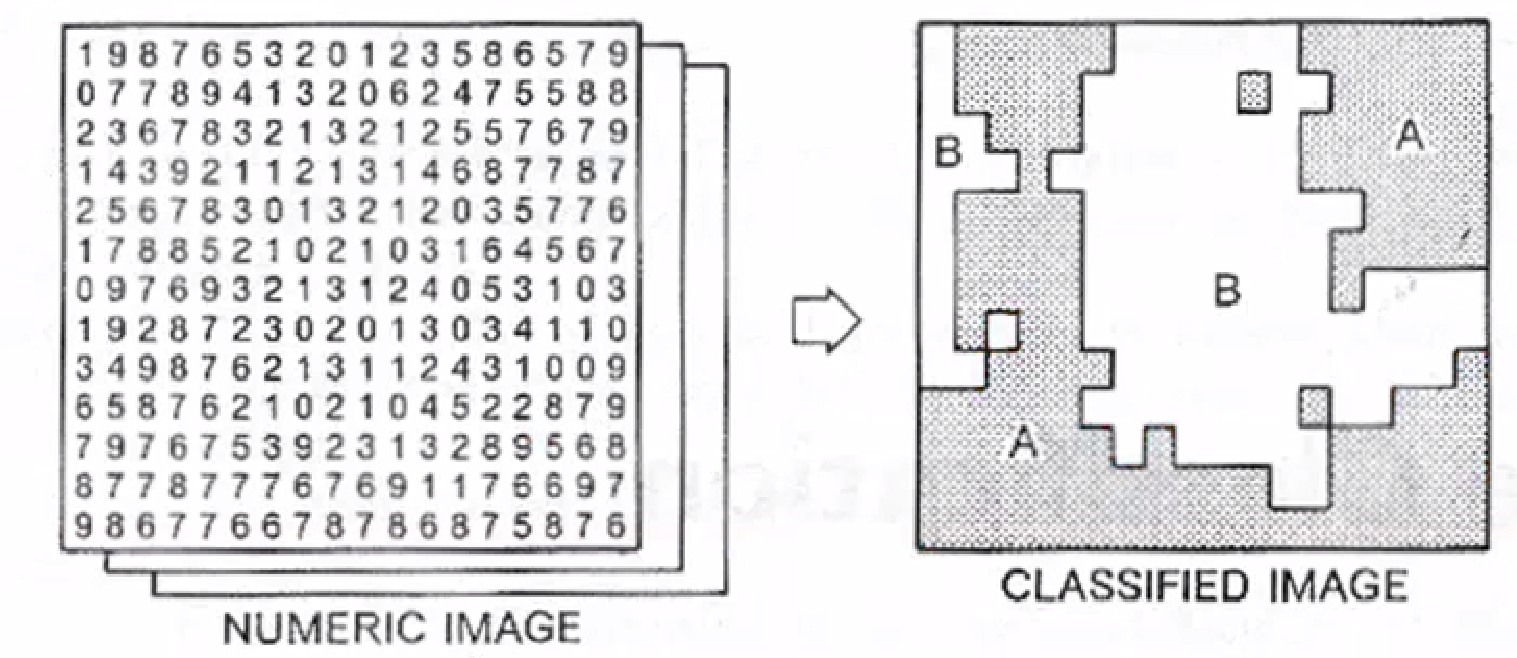
\includegraphics[width=0.5\textwidth]{t20.pdf}
    \caption{Imágen numérica e imagen clasificada. la imágen clasificada (derecha) es definida por la examinación de la imágen numérica, entonces agrupando los pixeles que tienen valores espectrales similares. La clase A es formado por el brillo de los pixeles (valores de 6,7. 8 y 9) y B es hecho por pixeles oscuros (valores de 0,1,2 y 3). Usualmente hay muchas más clases y al menos tres o cuatro bandas espectrales}
    \label{t20}
  \end{figure}
  
  \begin{definition}[Distribución de frecuencia]
      Es un método de resumir o de sintetizar grandes volúmenes de datos en un número limitado de clases o categorías
  \end{definition}
  
  \begin{definition}[Histrograma]
      Es una representación gráfica, en forma de barra, de una distribución de frecuencia. El Histograma de una imágen describe la distribución de los pixeles de una imagen en términos del número de píxeles para cada valor de DN\footnote{Se le recomienda al lector, que haga una revisión al capítulo de ``Métodos estadísticos'' del segundo semestre.}
      \begin{equation}
          Hist_{DN} = \frac{conteo(DN)}{N} 
      \end{equation}
  \end{definition}
  
  \begin{definition}[Histograma acumulativo]
      Es la proporción de píxeles en la imágen con DN menor o igual que un valor definido de DN
      \begin{equation}
          Hista_{DN} =\sum_{DN = 0}^{DN = 255} Hist_{DN}
      \end{equation}
  \end{definition}

Distancia espectral entre dos pixeles en una imagen de $k$ bandas espectrales:

\begin{align}
  d_{i,j} = \sqrt{ \sum_{1}^{k} \left(Dn_{i,j} - Dn_{i,j}\right)^2}\\
  d_{i,j} = \sqrt{ \sum_{1}^{k} \left(\mu_{i,k} - \mu_{j,k}\right)^2}
\end{align}

Donde $DN_{i,j}$ es el valor del pixel $i$ en la banda $k$, $DN_{j,k}$ es el valor del píxel $j$ en la misma banda $k$,
$k$ es el número de bandas, $\mu_{i,j}$ es la media de la clase espectral $i$ y $\mu_{j,k}$ es la media de la clase espectral $j$.

\begin{table}[h!]
  \centering\begin{tabular}{@{}llll@{}}
  \toprule
        & $P_1$      & $P_2$      & $P_3$      \\ \midrule
  $B_1$ & $\mu_{11}$ & $\mu_{21}$ & $\mu_{31}$ \\
  $B_2$ & $\mu_{12}$ & $\mu_{22}$ & $\mu_{32}$ \\
  $B_3$ & $\mu_{13}$ & $\mu_{23}$ & $\mu_{33}$ \\ \bottomrule
  \end{tabular}
  \caption{Diferencia espectral de los patrones}
  \label{tabt3}
  \end{table}

  La  fórmula para calcular la Divergencia  es una adaptación 
  de Swain et al. (1978):
  \begin{align*}
      D_{i,j} = 0.5 tr \left(COV_i - COV_j\right)\left(COV_i^{ -1} - COV_j^{ - 1}\right) + 0.5tr\left(COV_i^{ 1} - COV_j^{ - 1}\right)\left(M_i - M_j\right)\left(M_i - M_j\right)^{T}
  \end{align*}
  
  Donde $i$, $j$ firmas espectrales (o clases) a comparar, $COV_i$
  es la matriz de covarianza de la firma o clase espectral i,
  $M_i$ el vector medio de la firma espectral  i,
  $tr$ la función función  traza (álgebra de matrices) y 
  $T$ la función de  transposición.
  
  
  La  geoestadística aplicada al análisis de las imágenes mide la 
      similaridad espacial de los pares de valores DN localizados a 
      una distancia h.
  
      La tasa de cambio promedio de pares de DN localizados en 
      $i$ e $i+h$ puede ser estimada calculando su semivarianza de     
  acuerdo con la siguiente expresión:
  \begin{equation}
      \gamma(h)\, \frac{1}{2N(h)}\sum_{i=1}^{N(h)} \left(DN_{i} - DN_{i + h}\right)^2
  \end{equation}
  
  Donde $\gamma(h)$ es la semivarianza, 
  $N(h)$ es el número de pares a una distancia dada $h$, 
  $DN_i$ el valor DN en un punto $i$,  
  $Z_i + h$ es el valor de DN a una distancia h de i. 
  
  La covarianza y la semivarianza se relacionan con la siguiente relación
  \begin{equation}
      \gamma(h) = COV_0 - COV_h
  \end{equation}
  
  La semivarianza ha sido considerada como una medida de la 
  similitud entre observaciones situadas a una determinada 
  distancia del lugar i, ya que mientras más similares sean las 
  observaciones menor es la semivarianza
  
  Semivariograma: El gráfico de la semivarianza contra la distancia, es conocido como 
  Semivariograma.
  
  \begin{figure}[h!]
  \centering
    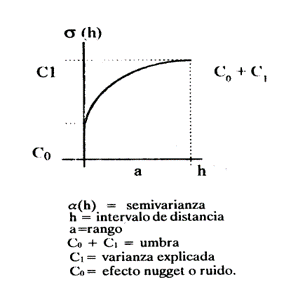
\includegraphics[width=0.5\textwidth]{t21.png}
    \caption{Semivariograma}
    \label{t21}
  \end{figure}
  Según Journel y Huigbregts (1978 ) se debe estimar cada punto de 
  semivarianza con al menos 30 pares de observaciones para construir 
  un semivariograma confiable. 
  
  Webster y Oliver (1992) expresan que la precisión de la estimación del 
  semivariograma está condicionada más bien por el número total de 
  observaciones que componen la muestra y consideran que 50 
  observaciones es un número de muestras muy pequeño y que al menos 
  100 observaciones son necesarias, pero 150 datos podrían ser 
  satisfactorios para una variable isotrópicamente distribuida, mientras 
  que uno derivado de 225 usualmente sería más confiable.
  
  \subsection{Rectificación de la imagen}
  
  Es el proceso de georeferenciación de una imagen para que se ajuste a un sistema de proyección dada.
  
  Rectificar los píxeles del sistema de grid de la imagen para ajustarlos a los sistemas de proyección de un mapa o  de una imagen rectificada. Estos documentos son  considerados como referencias.
  
  La georeferenciación es requerida para la realización de varias operaciones de SIG como 
  la elaboración de fotomapas,  sobreposición de vectores 
  sobre imágenes, elaboración de mosaicos, 
  comparación de imágenes con diferentes escalas 
  originales.
  
  Los etapas de la rectificación son tres:
  \begin{enumerate}
      \item Localizar los puntos de control terrestres tanto en la imagen como en el documento de referencia
      \item Calcular y probar la matriz de transformación
      \item Crear la imagen corregida resultante
  \end{enumerate}
  
  \subsubsection{Ajustes polinomiales}
  
  Las variables ($x, y$), y coeficientes. 
  las ecuaciones polinomiales son expresiones matemáticas que La forma general de un polinomio es para una variable:
  \begin{equation}
      A + Bx + Cx^2 + Dx^3 +\dots +\Omega x^t
  \end{equation}
  para dos variables, $i+j\leq 1$
  \begin{equation}
      A + Bx + Cy + Dx^2 + Fy^2+\dots + Qx^iy^j +\dots +\Omega x^t
  \end{equation}
  
  Los puntos de controles terrestres de una imagen fuente son 
  transformadas en coordenadas reales mediante un ajuste 
  polinomial.  

  Las ecuaciones anteriores pueden escribirse de la siguiente forma:
  \begin{equation}
    \begin{bmatrix}
        x_0\\ y_0
    \end{bmatrix} =\begin{bmatrix}
        a_{10}a_{01} &a_{ij}&a_{t0}  \\
        b_{10}b_{01}&b_{ij}&b_{t0}  
    \end{bmatrix}\begin{bmatrix}
         x \\
         Y  
    \end{bmatrix} +\begin{bmatrix}
        a_{00}\\ b_{00}
    \end{bmatrix}
\end{equation}
La cual es equivalente a:
\begin{equation}
    p = Tp_{ref} + T_0
\end{equation}
\begin{table}[h!]
  \centering \begin{tabular}{@{}ll@{}}
    \toprule
    Coeficientes & Contribución                    \\ \midrule
    $a_{00}$          & Desplazamiento en x             \\
    $b_{00}$          & Desplazamiento en y             \\
    $a_{10}$          & Escala en x                     \\
    $b_{01}$          & Escala en y                     \\
    $a_{01}$          & Torcedura en x                  \\
    $b_{10}$          & Torcedura en y                  \\
    $a_{11}$          & Dependencia de la escala y en x \\
    $b_{11}$          & Dependencia de la escala x en y \\
    $a_{20}$          & Escala no lineal en x           \\
    $b_{02}$          & Escala no lineal en y           \\ \bottomrule
    \end{tabular}
    \caption{Contribución de cada coeficiente en la ecuación polinomial}
    \label{tabt4}
    \end{table}

    Transformaciones afines:
    Esta última ecuación puede ser usada para realizar diversas 
    correcciones aproximadas de las distorsiones del sensor de 
    Satélite así como distorsiones orbitales.
    La matrices de transformaciones individuales pueden ser 
    Combinadas en una solo:
    
    \begin{table}[h!]
      \centering\begin{tabular}{@{}ll@{}}
        \toprule
        Distorsión            & Matriz de Transformación                                                                                                                                                      \\ \midrule
        Aspecto proporcional  & \begin{tabular}[c]{@{}l@{}}$T_1 = \begin{bmatrix}\\         1 & 0 \\\\         0 & 0.709 \\     \end{bmatrix}$\end{tabular}                                                   \\
        Rotación de la Tierra & \begin{tabular}[c]{@{}l@{}}$T_2 = \begin{bmatrix}\\         1 & -\alpha \\\\         0 & 1 \\     \end{bmatrix},\alpha = \tan{(\gamma)}\cos{(\psi)}\cos{\theta}$\end{tabular} \\
        Rotación al Norte     & \begin{tabular}[c]{@{}l@{}}$T_3 = \begin{bmatrix}\\         \cos{\theta} & -\sin{\theta} \\\\         \sin{\theta} &\cos{\theta}  \\     \end{bmatrix}$\end{tabular}          \\ \bottomrule
        \end{tabular}
        \caption{$T_{total}=T_1T_2T_3$}
        \label{tabt5}
    \end{table}
    El número de coeficientes contenido dentro de una matriz de 
    Transformación  es función del orden del polinomio: $(t+1)(t+2)$    

    Número mínimo de Puntos de control terrestre:
\begin{equation}
    \frac{(t+1)(t+2)}{2}
\end{equation}
Raíz Cuadrada media del Error: RMS error
\begin{equation}
    RMS_{error} = \sqrt{\left(x_r - x_i\right)^2 +\left(y_r - y_i\right)^2}
\end{equation}

Corrección Radiométrica por Faja de vuelo (Chavez, P. S., Jr., 1996 )
\begin{equation}
    L = Graom\cdot DN + offset
\end{equation}
Donde: $L$ =  Radiancia espectral  media de la banda espectral, $DN$ = Valor del Número digital registrado, $Grain$ =  $\frac{(L_{max} - L_{min})}{(2^{12}-1)}$  pendiente de la función de respuesta, $Offset$ =  $L_{min}$, $L_{max}$ =  radiancia medida en la saturación del detector en $mWcm^2sr^{-1}$
      $L_{min}$ =  la más baja radiación medida por el detector en $mWcm^{-2}sr^{-1}$
La reflectancia en una banda determinada es calculada en la ecuación:
\begin{equation}
    Re\cdot flec \cdot\tan{cia} =\left(\frac{\pi\cdot d^2}{E\sin{(\alpha)}}\right)L
\end{equation}
Donde: $E$ =  Irradiancia en el tope de la atmósfera en $mWcm^{-2}$ 
$\alpha$ =  Elevación solar

\subsubsection{Filtraje Direccionales}
Es un caso particular de filtraje de 
alta frecuencia usado para resaltar rasgos lineales con 
orientación preferencial.
\begin{table}[h!]
  \centering\begin{tabular}{@{}ccccc@{}}
    \toprule
    Vertical                                                                                            & Horizontal                                                                                            & \multicolumn{2}{c}{Diagonal}                                                                                                                                                                                                          & Azimutal                                                                                                                                                                   \\ \midrule
    \begin{tabular}[c]{@{}c@{}}$\begin{bmatrix*}\\         - 1&+ 1\\     \end{bmatrix*}$\end{tabular}   & \begin{tabular}[c]{@{}c@{}}$\begin{bmatrix*}\\         - 1\\1\\     \end{bmatrix*}$\end{tabular}      & \begin{tabular}[c]{@{}c@{}}$\begin{bmatrix*}\\         0&- 1\\1&0\\     \end{bmatrix*}$\end{tabular}              & \begin{tabular}[c]{@{}c@{}}$\begin{bmatrix*}\\         - 1&0\\ 0&1\\     \end{bmatrix*}$\end{tabular}             & \begin{tabular}[c]{@{}c@{}}$\begin{bmatrix*}\\         \sin{(\alpha)}&0\\\\         -\sin{(\theta)} - \cos{(\theta)} & \cos{(\theta)}\\\\     \end{bmatrix*}$\end{tabular} \\
    \begin{tabular}[c]{@{}c@{}}$\begin{bmatrix*}\\         - 1&2 &-1\\     \end{bmatrix*}$\end{tabular} & \begin{tabular}[c]{@{}c@{}}$\begin{bmatrix*}\\         - 1\\2\\- 1\\     \end{bmatrix*}$\end{tabular} & \begin{tabular}[c]{@{}c@{}}$\begin{bmatrix*}\\         0&0&- 1\\0&2&0\\- 1&0&0\\     \end{bmatrix*}$\end{tabular} & \begin{tabular}[c]{@{}c@{}}$\begin{bmatrix*}\\         - 1&0&0\\0&2&0\\0&0&- 1\\     \end{bmatrix*}$\end{tabular} &                                                                                                                                                                            \\ \bottomrule
    \end{tabular}
    \caption{Filtraje Direccionales}
    \label{tabt6}
    \end{table}

\subsubsection{Filtros de gradientes}

Permiten resaltar los cambios significativos en valores DN de 
un píxel a otro. Estos cambios corresponden a linderos, caminos, líneas de costas, etc.

\begin{table}[h!]
  \centering\begin{tabular}{@{}lll@{}}
    \toprule
    Filtro  & Componente Horizontal                                                                                                                                  & Componente Vertical                                                                                                                                     \\ \midrule
    Robert  & \begin{tabular}[c]{@{}l@{}}$\begin{bmatrix}\\         0 & 1 \\\\         - 1 & 0 \\     \end{bmatrix}$\end{tabular}                                    & \begin{tabular}[c]{@{}l@{}}$\begin{bmatrix}\\         1 & 0 \\\\         0 & - 1 \\     \end{bmatrix}$\end{tabular}                                     \\
    Sobel   & \begin{tabular}[c]{@{}l@{}}$\begin{bmatrix}\\         1 & 2 & 1\\\\         0 & 0 & 0\\\\         - 1&- 2&- 1\\     \end{bmatrix}$\end{tabular}        & \begin{tabular}[c]{@{}l@{}}$\begin{bmatrix}\\         -1  & 0 & 1\\\\         - 2 & 0 & 2\\\\         - 1 &0  & 1\\     \end{bmatrix}$\end{tabular}     \\
    Prewitt & \begin{tabular}[c]{@{}l@{}}$\begin{bmatrix}\\         1  & 1 & 1\\\\         1 & - 2 & 1\\\\         - 1 & - 1 & - 1\\     \end{bmatrix}$\end{tabular} & \begin{tabular}[c]{@{}l@{}}$\begin{bmatrix}\\         - 1  & 1 & 1\\\\         - 1 & - 2 & 1\\\\         - 1 & 1 &  1\\     \end{bmatrix}$\end{tabular} \\ \bottomrule
    \end{tabular}
    \caption{Filtros de gradientes}
    \label{tabt7}
    \end{table}

REPRESENTACIÓN ESPACIAL FIGURATIVA DE LA IMAGEN (Feature Space Image: FSI)
    
    Es la representación gráfica de los valores DN de una banda con 
    respecto a los valores DN de otra banda de la misma imagen.
    Por ejemplo: la banda 2 contra la banda 4
    
    \begin{figure}[h!]
        \centering
        \begin{subfigure}[b]{0.45\linewidth}
        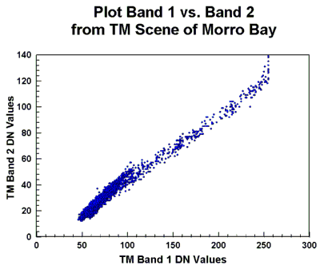
\includegraphics[width=\linewidth]{t22.png}
        \caption{Gráfico de la banda 1 vs banda 2 desde la TM scene del Morro Bay}
        \label{t22}
        \end{subfigure}
        \begin{subfigure}[b]{0.45\linewidth}
        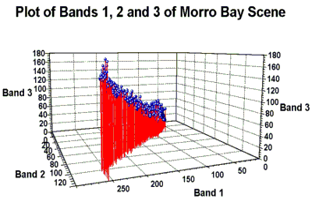
\includegraphics[width=\linewidth]{t23.png}
        \caption{Gráfica de la banda 1,2 y 4 del Morro Bay Scene}
        \label{t23}
        \end{subfigure}
        \caption{Palacio de Westminster}
        \label{t22-23}
        \end{figure}


        \subsection{Indices multiespectrales}

        \begin{equation}
            IV = \frac{\rho_{IRC}}{\rho_{Rojo}}\text{Índice de Vegetación}
        \end{equation}
        
        \begin{equation}
            NVDI =\frac{\rho_{IRC} -\rho_{Rojo}}{\rho_{IRC} +\rho_{Rojo}}\text{ Diferencia normal del I.V.}
        \end{equation}
        
        \begin{equation}
            SAVI =\left(\frac{\rho_{IRC} -\rho_{Rojo}}{\rho_{IRC} +\rho_{Rojo} + L}\right)\left(1 + L\right)\text{Ajuste del suelo I.V.}
        \end{equation}
        
        Si $L=0\implies SAVI=NVDI$, cuando $L=0.5$, es un suelo moderadamente cubierto de vegetación y $1+L$ asegura que $SAVI$ varía entre -1 y 1.
        

        \subsubsection{Componentes principales}

        Las bandas espectrales de las imágenes están altamente 
        correlacionadas causadas por una combinación de factores:
        \begin{itemize}
            \item Baja reflectancia de la vegetación en todo el visible
            \item La topografia y el bajo angulo solar influyen sobre el  patrón de sombra que afecta todo el espectro EM
            \item La sobreposición de las bandas del sensor (controlable)
        \end{itemize}
        
        Las transformaciones de componentes principales fueron 
        diseñadas para eliminar la redundancia espectral.
        
        El análisis de CP (o PC in inglés) se basa en una combinación
        linear de todos los elementos para cada vector pixel de la 
        imagen.
        \begin{equation}
            PC_{i,j,1} = a_{(i,j,1)}DN_{(i,j,1)} + a_{(i,j,2)} + \dots + a_{(i,j,k)}DN_{(i,j,k)}
        \end{equation}
        La ecuación general de transformación lineal para calcular el 
        principal componente es:
        \begin{equation}
            PC = W_{PC}\cdot DN
        \end{equation}
        La relación entre covarianza de la imagen PC y la matriz de
        covarianza de la imagen original se muestra en la siguiente 
        ecuación:
        \begin{equation}
            COV_{PC} = COV\dot W_{PC}T
        \end{equation}
        De todos los $W_{PC}$ calculados se selecciona el $W_{PC}$  que 
        Diagonaliza la matriz de covarianza de la imagen original 
        
        Esta transformación es una rotación de los ejes originales hacia 
        nuevas  orientaciones que son ortogonales entre sí de modo que
        No hay correlación entre variables.






